\documentclass{article}
\usepackage{graphicx} % Required for inserting images
\usepackage[margin=2cm, top=3cm]{geometry} % margine superiore ridotto a 1 cm
\usepackage{listings}
\usepackage{subcaption}  % Pacchetto per sottodidascalie
\usepackage{float}       % Pacchetto per posizionamento rigido delle figure
\usepackage{amsmath}
\title{Intelligenza Artificiale e Machine Learning preparazione all'Esonero}
\author{Mattia Cosimi}
\date{November 2024}

\begin{document}

\maketitle
\section{Problem Solving e Search}
\subsection{Introduzione}
Il processo di ricerca comporta i seguenti passi: scegliere (tra le foglie dell'albero) un nodo da "espandere", secondo una strategia. Controllare se il nodo scelto è un obiettivo, se non lo è, "espandere" il nodo: generare i suoi figli, ciascuno dei quali contiene uno stato risultante dall'applicazione di un operatore allo stato del nodo espanso.
La collezione di nodi in attesa di essere espansi è chiamata \textbf{frontiera}. La frontiera è implementata da una struttura che chiamiamo "coda" (queue).
\subsection{Tree Search}
\begin{figure}[H] % Usa 'H' per forzare la posizione qui
    \centering % Centra l'immagine
    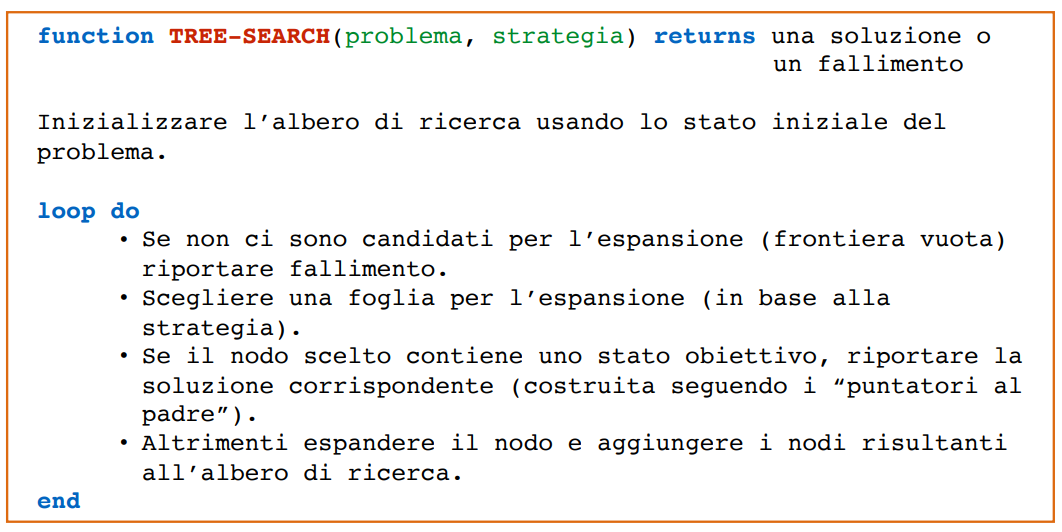
\includegraphics[width=12cm, height=5cm]{immagine_2024-11-09_180136244.png} % Percorso dell'immagine
    %\caption{Tree Search} % Didascalia per l'immagine
    \label{fig:immagine} % Etichetta per riferimento
\end{figure}
\begin{figure}[H] % Usa 'H' per forzare la posizione qui
    \centering % Centra l'immagine
    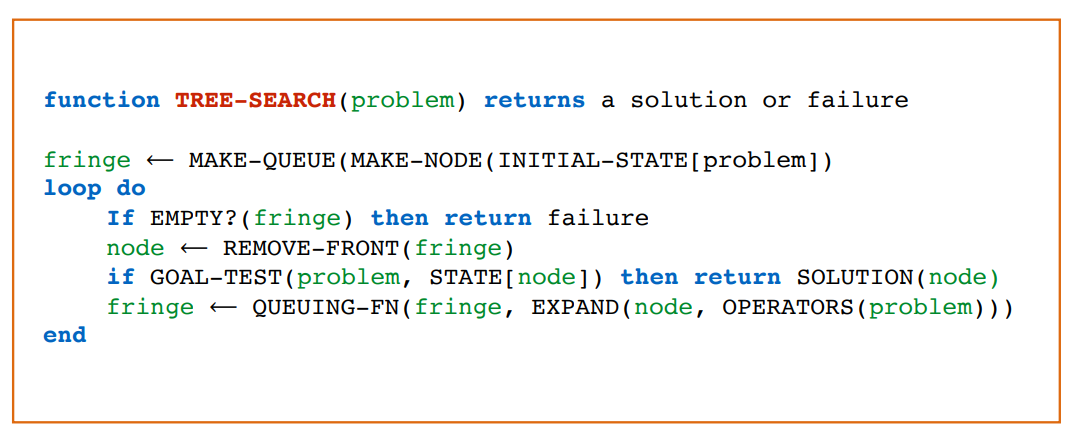
\includegraphics[width=12cm, height=5cm]{immagine_2024-11-09_180519152.png} % Percorso dell'immagine
    %\caption{Tree Search} % Didascalia per l'immagine
    \label{fig:immagine} % Etichetta per riferimento
\end{figure}
\vspace{20pt}
\section{Ricerca Cieca}
\subsection{Ricerca in Ampiezza (Breadth-First-Search)}
Si espande il nodo radice, si espandono i nodi generati dalla radice, si espandono i loro successori e cosi via.
\begin{figure}[H] % Usa 'H' per forzare la posizione qui
    \centering % Centra l'immagine
    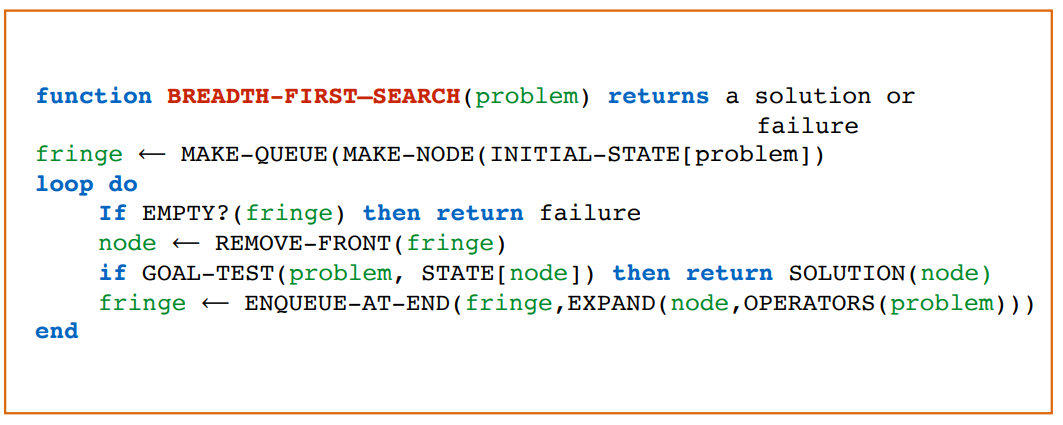
\includegraphics[width=12cm, height=5cm]{immagine_2024-11-09_182539144.png} % Percorso dell'immagine
    %\caption{Tree Search} % Didascalia per l'immagine
    \label{fig:immagine} % Etichetta per riferimento
\end{figure}
\begin{figure}[htbp]
    \begin{minipage}[b]{0.45\textwidth} % Prima figura a sinistra
        \centering
        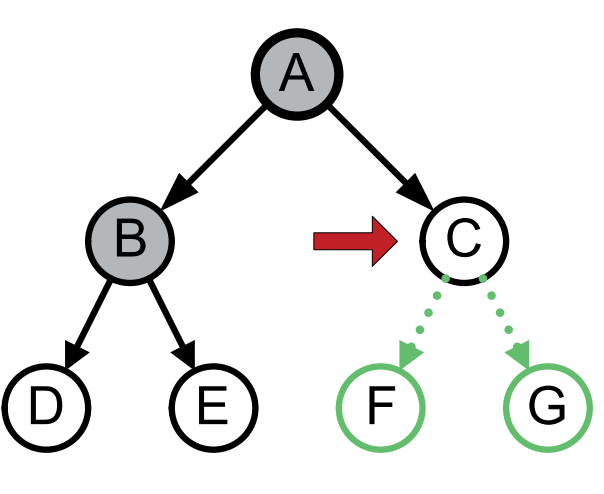
\includegraphics[width=6cm, height=6cm]{Screenshot 2024-11-09 182105.png} % Sostituisci con il nome del tuo file immagine
        %\caption{Tree Search}
    \end{minipage}
    \hfill
    \begin{minipage}[b]{0.45\textwidth} % Seconda figura a destra
        \centering
        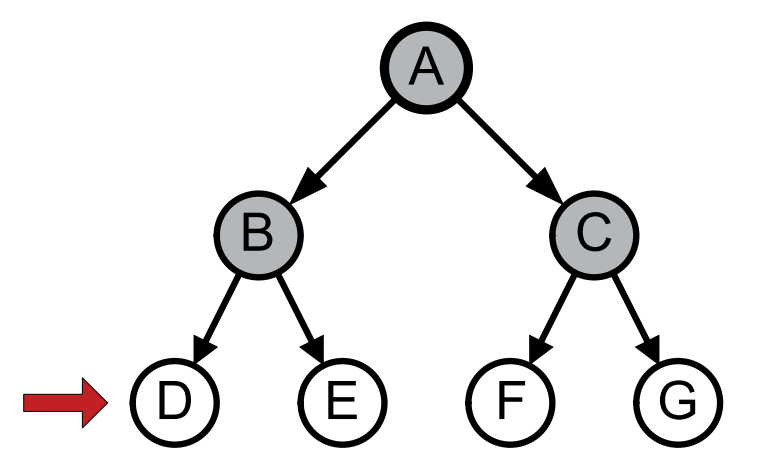
\includegraphics[width=7cm, height=6cm]{Screenshot 2024-11-09 182121.png} % Sostituisci con il nome del tuo file immagine
        %\caption{Graph Search}
    \end{minipage}
\end{figure}
\noindent
Trova sicuramente la soluzione realizzabile con il cammino più breve, ma il cammino più breve non è necessariamente quello a costo minimo. È \textbf{completo}. È \textbf{ottimale} se il costo del cammino è una funzione monotona non decrescente della profondità del nodo. La \textbf{Complessità in tempo e in spazio:} $O(b^d)$ dove b è il fattore di ramificazione dell'albero (ogni nodo ha al massimo b figli) e d è la lunghezza minima di un cammino dal nodo iniziale alla soluzione.
\subsection{Ricerca guidata dal costo}
Modifica la ricerca in ampiezza espandendo il nodo nella frontiera con costo più basso. $g(n)$ è il costo dalla radice a n. È completo e ottimale se il costo di ogni step $(g(successor(n)) - g(n))$ è sempre maggiore o uguale a una costante positiva.
\vspace{80pt}
\subsection{Ricerca in profondità (Depth-First-Search)}
Nella ricerca in profondità si procede come segue: si espande il nodo radice, si procede espandendo sempre per primo il nodo più profondo nella frontiera corrente dell'albero di ricerca.
\begin{figure}[H] % Usa 'H' per forzare la posizione qui
    \centering % Centra l'immagine
    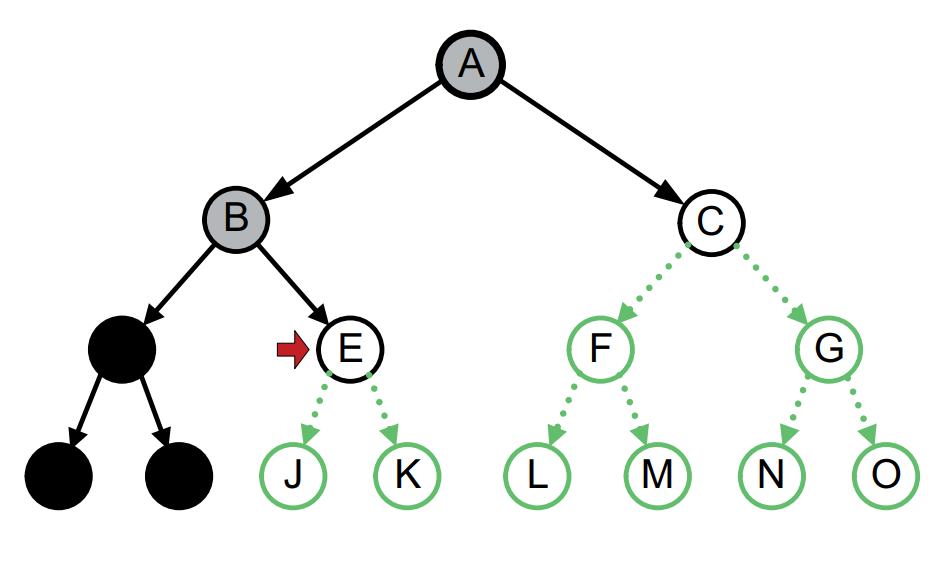
\includegraphics[width=10cm, height=5cm]{Screenshot 2024-11-10 152410.png} % Percorso dell'immagine
    %\caption{Tree Search} % Didascalia per l'immagine
    \label{fig:immagine} % Etichetta per riferimento
\end{figure}
\begin{figure}[H] % Usa 'H' per forzare la posizione qui
    \centering % Centra l'immagine
    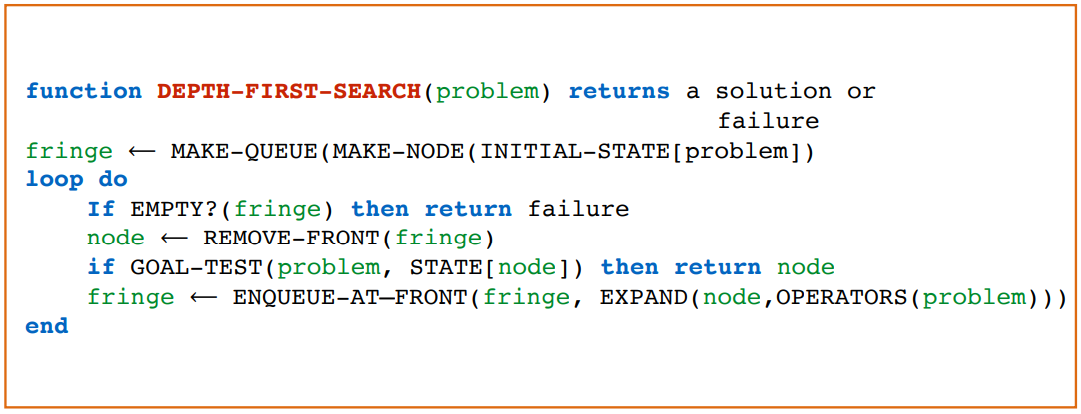
\includegraphics[width=14cm, height=5cm]{immagine_2024-11-10_152701570.png} % Percorso dell'immagine
    \caption{Depth-First Search} % Didascalia per l'immagine
    \label{fig:immagine} % Etichetta per riferimento
\end{figure} 
\noindent
Quando si espande un nodo non obiettivo e senza figli, si fa backtracking ovvero si torna indietro fino all'ultimo nodo in cui è possibile effettuare una scelta. Non è ne \textbf{completa} ne \textbf{ottimale}. Complessità in tempo O($b^m$) dove m è la profondità massima dell albero di ricerca. Complessità in spazio $O(b\cdot m)$
\subsection{Ricerca in profondità limitata}
Opera come la ricerca in profondità imponendo, però, un limite alla profondità massima dei cammini: un nodo viene espanso solo se la lunghezza del cammino corrispondente è minore del massimo stabilito. Se non viene trovata alcuna soluzione l'algoritmo restituisce il valore speciale taglio se alcuni nodi non sono stati espansi per il limite della profondità, altrimenti fallimento. È \textbf{completa se} il problema è tale che, se ha soluzione, allora esiste una soluzione di lunghezza minore o uguale al limite massimo. Non è \textbf{ottimale}. Complessità in tempo O($b^l$) dove l è il limite di profondità fissato. Complessità in spazio O($b \cdot l$)
\vspace{80pt}
\subsection{Ricerca per approfondimenti successivi (Iterative-Deepening Search)}
Non sempre si conosce un limite adeguato per la ricerca in profondità limitata. Questa strategia evita il problema della scelta di un limite adeguato provando iterativamente tutti i limiti possibili.
\begin{figure}[H] % Usa 'H' per forzare la posizione qui
    \centering % Centra l'immagine
    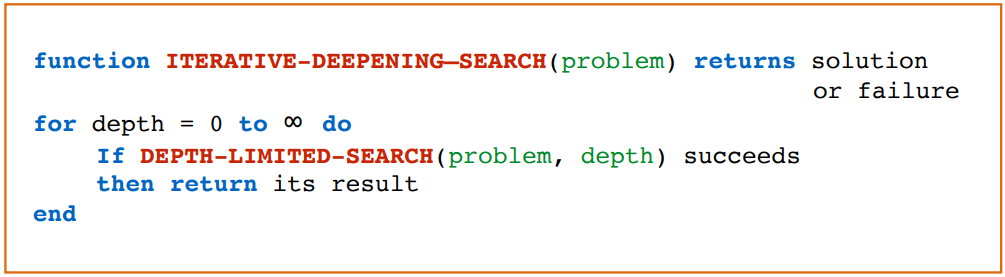
\includegraphics[width=14cm, height=4cm]{Screenshot 2024-11-10 154255.png} % Percorso dell'immagine
    \caption{Iterative-Deepening Search} % Didascalia per l'immagine
    \label{fig:immagine} % Etichetta per riferimento
\end{figure} 
\noindent
\textbf{È completa e ottimale} (sotto le stesse ipotesi della ricerca in ampiezza). Complessità in spazio O($b \cdot d)$ dove d è la profondità minima di una soluzione. Complessità in tempo O($b^d$).
\subsection{Graph Search}
Nasce dall'esigenza di evitare la ripetizione degli stati. Per questo al tree search viene aggiunta una lista chiusa che ci permette di memorizzare i nodi già visitati.
\begin{figure}[H] % Usa 'H' per forzare la posizione qui
    \centering % Centra l'immagine
    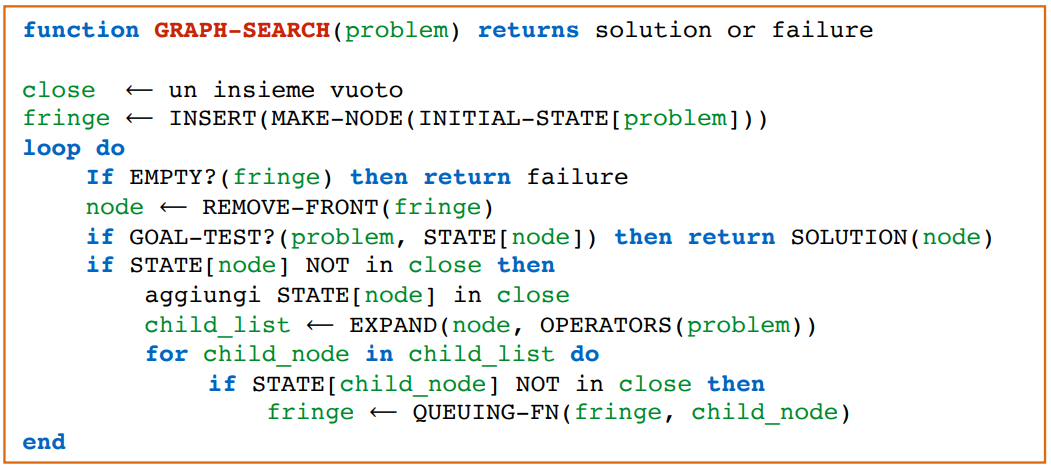
\includegraphics[width=14cm, height=6cm]{immagine_2024-11-10_155204453.png} % Percorso dell'immagine
    \caption{Graph Search} % Didascalia per l'immagine
    \label{fig:immagine} % Etichetta per riferimento
\end{figure} 
\noindent
\section{Ricerca Euristica}
\subsection{Introduzione}
La parola euristica significa, che aiuta nella scoperta. Infatti nell'algoritmo GENERAL-SEARCH si può usare conoscenza euristica per definire la QUEUING-FUNCTION ovvero ciò che determina la scelta del nodo da espandere. La conoscenza sul problema è rappresentata da una \textbf{funzione di valutazione} che si applica ai nodi dell albero di ricerca, in particolare f(nodo)= stima della desiderabilità di espandere il nodo; misura di quanto il nodo è promettente. Normalmente f è una stima del costo della soluzione, quindi viene considerato migliore il nodo n con f(n) minore.
\subsection{Best-First Search}
La QUEUING-FN ordina i nodi dal migliore al peggiore secondo la funzione di valutazione. Il nodo scelto per l'espansione è quello la cui valutazione è migliore, cioè il nodo apparentemente più promettente. 
\begin{figure}[H] % Usa 'H' per forzare la posizione qui
    \centering % Centra l'immagine
    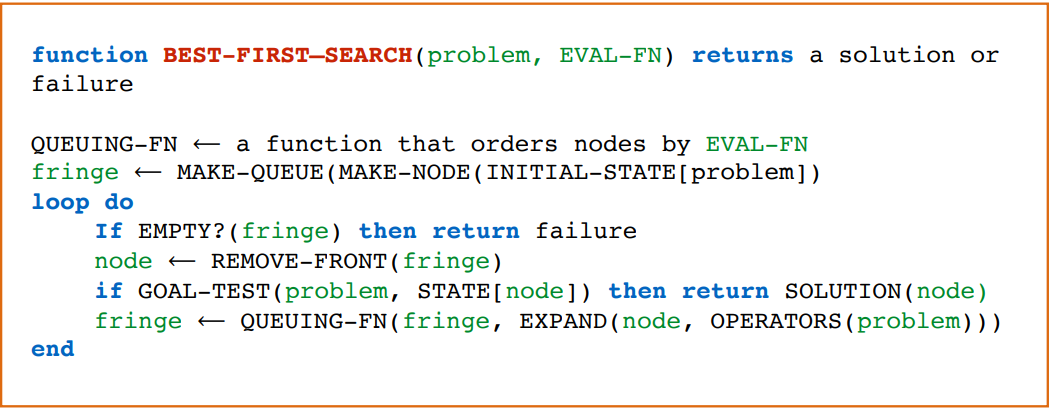
\includegraphics[width=14cm, height=5cm]{Screenshot 2024-11-07 170219.png} % Percorso dell'immagine
    \caption{Best-First Search} % Didascalia per l'immagine
    \label{fig:immagine} % Etichetta per riferimento
\end{figure}
\vspace{-20pt}
\begin{figure}[H] % Usa 'H' per forzare la posizione qui
    \centering % Centra l'immagine
    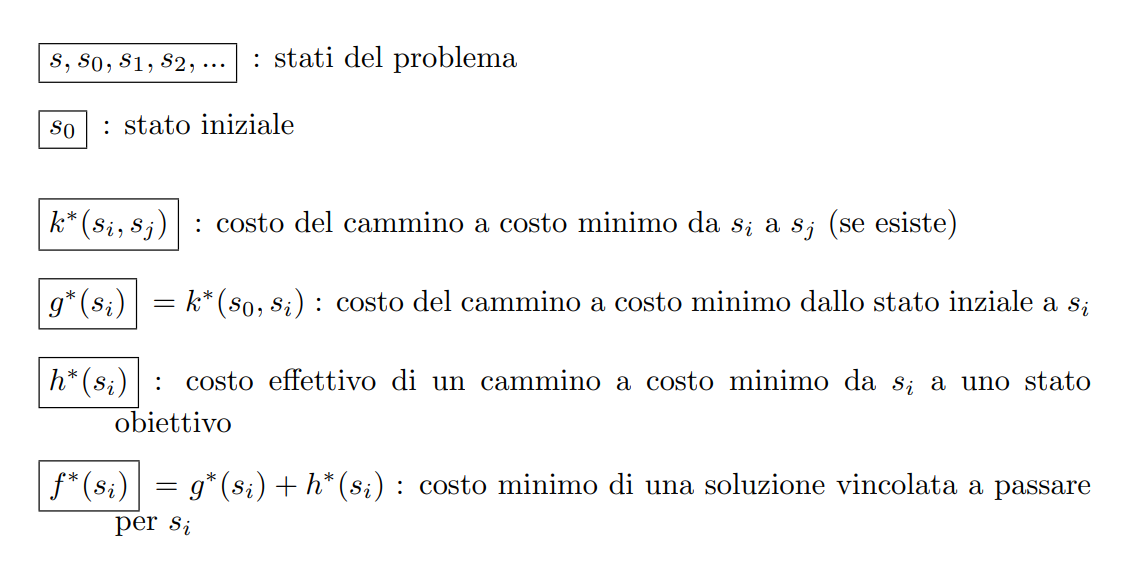
\includegraphics[width=12cm, height=5cm]{immagine_2024-11-07_171045739.png} % Percorso dell'immagine
    \caption{Notazioni (1)} % Didascalia per l'immagine
    \label{fig:immagine} % Etichetta per riferimento
\end{figure}
\begin{figure}[H] % Usa 'H' per forzare la posizione qui
    \centering % Centra l'immagine
    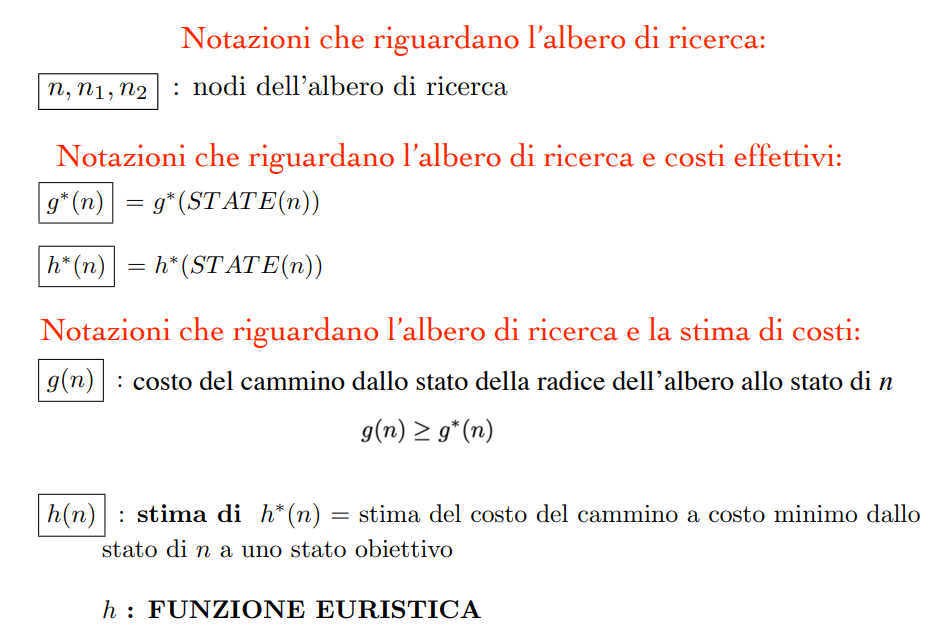
\includegraphics[width=12cm, height=6cm]{immagine_2024-11-07_171217725.png} % Percorso dell'immagine
    \caption{Notazioni (2)} % Didascalia per l'immagine
    \label{fig:immagine} % Etichetta per riferimento
\end{figure}
\noindent
\subsection{Greedy Best-First Search}
Ha una \textbf{Funzione di valutazione} $f=h$ che espande il nodo ritenuto più vicino a un obiettivo. Se h(n) = 0 vuol dire che lo stato n è un obiettivo. La ricerca golosa minimizza il costo stimato per raggiungere l'obiettivo.
\subsubsection{Esempio (Ricerca Itinerario)}
L'obiettivo è quello di raggiungere Bucarest a partire da Arad cercando di minimizzare il percorso.
\begin{figure}[H] % Usa 'H' per forzare la posizione qui
    \centering % Centra l'immagine
    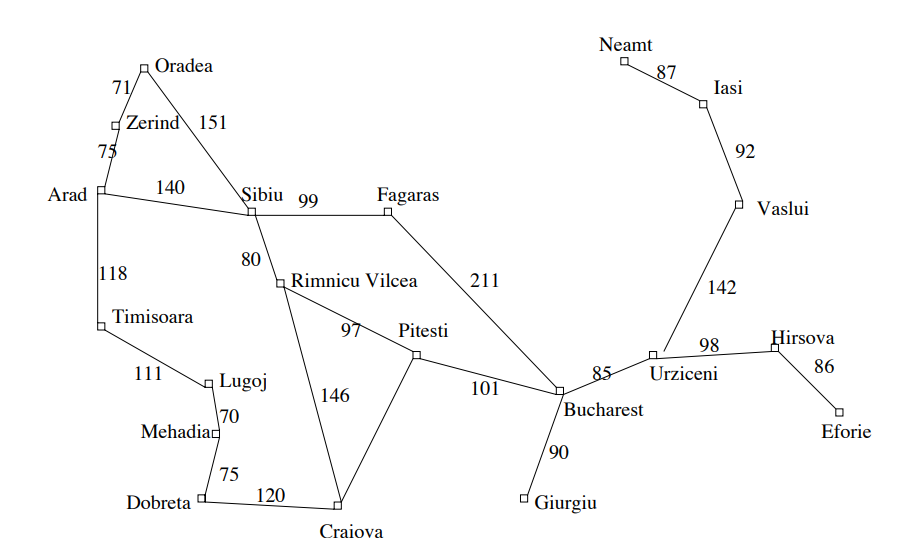
\includegraphics[width=12cm, height=6cm]{immagine_2024-11-07_171828243.png} % Percorso dell'immagine
    \caption{Mappa della Romania} % Didascalia per l'immagine
    \label{fig:immagine} % Etichetta per riferimento
\end{figure}
\begin{figure}[H] % Usa 'H' per forzare la posizione qui
    \centering % Centra l'immagine
    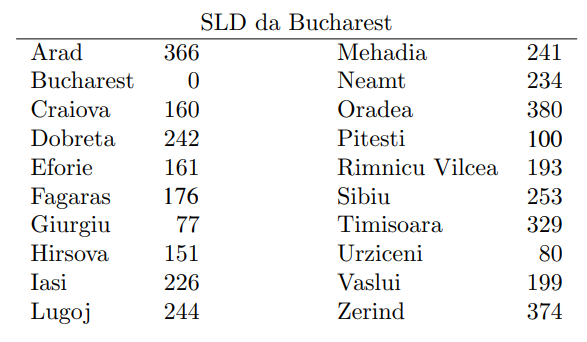
\includegraphics[width=12cm, height=6cm]{Screenshot 2024-11-07 173805.png} % Percorso dell'immagine
    \caption{SLD da Bucarest} % Didascalia per l'immagine
    \label{fig:immagine} % Etichetta per riferimento
\end{figure}
h=h$_{\text{SLD}}$(n) = distanza in linea d'aria (Straight Line Distance) dallo stato in n all'obiettivo
\begin{figure}[H] % Usa 'H' per forzare la posizione qui
    \centering % Centra l'immagine
    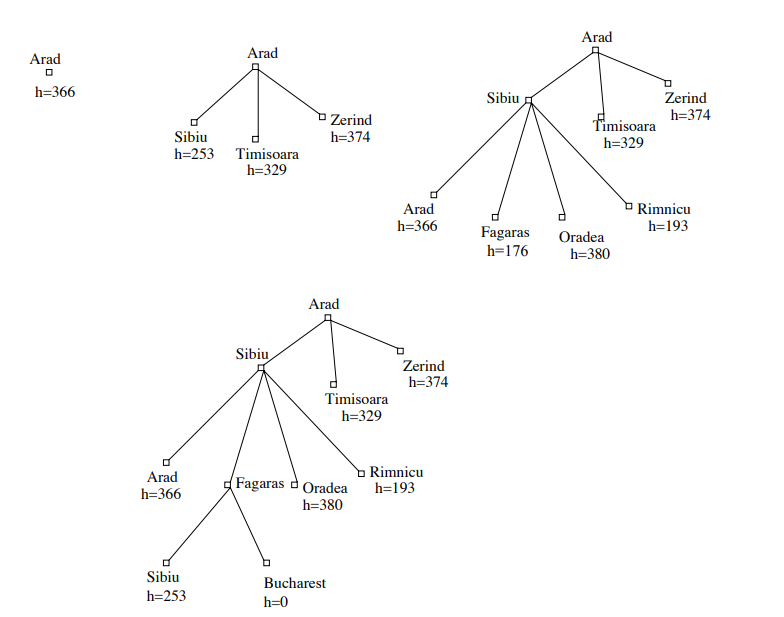
\includegraphics[width=13cm, height=8cm]{immagine_2024-11-07_172321913.png} % Percorso dell'immagine
    \caption{Ricerca golosa con funzione euristica h=h$_{\text{SLD}}$} % Didascalia per l'immagine
    \label{fig:immagine} % Etichetta per riferimento
\end{figure}
Il problema è che questo tipo di ricerca non ci porta alla soluzione ottima. Quindi \textbf{non è completa}, infatti potremmo seguire un cammino infinito senza trovare mai la soluzione e \textbf{non è ottimale}.
\subsubsection{Greedy Best-First Search codice Python}
\begin{figure}[H] % Usa 'H' per forzare la posizione qui
    \centering % Centra l'immagine
    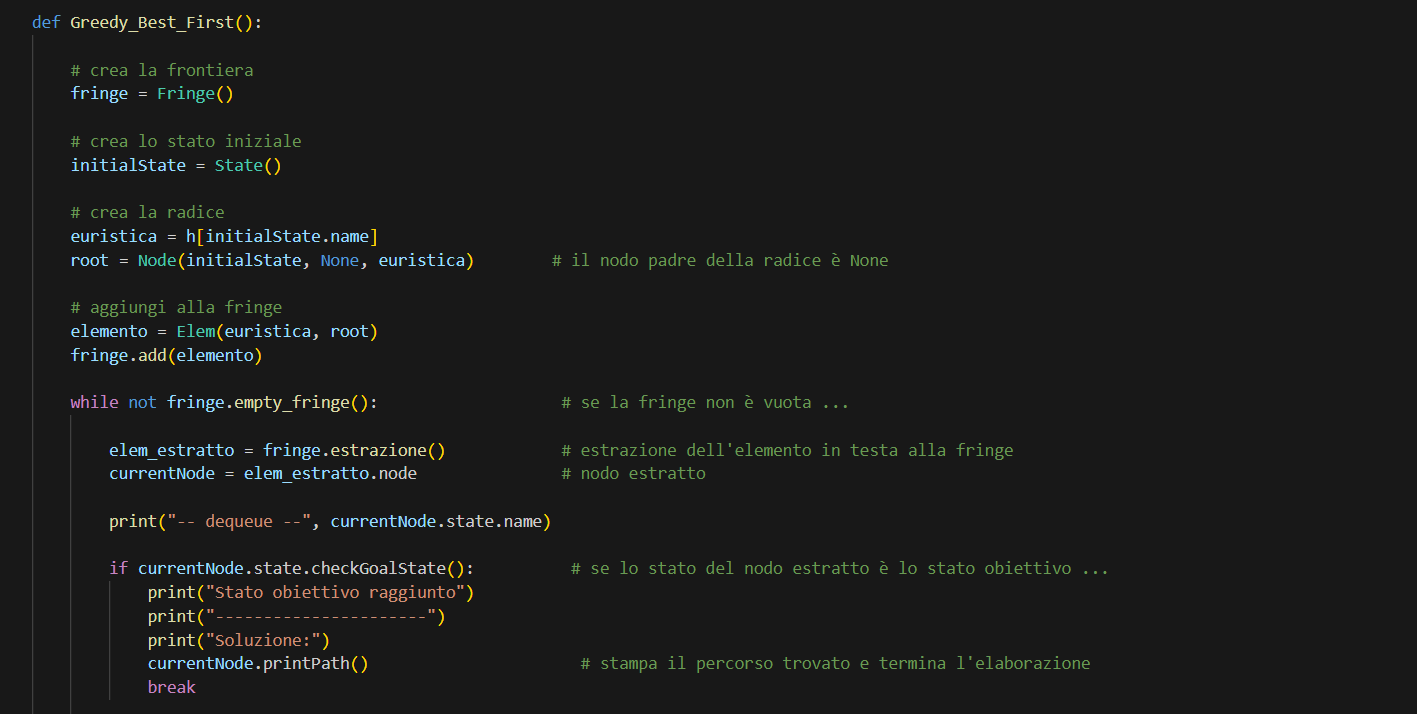
\includegraphics[width=18cm, height=10cm]{Screenshot 2024-11-10 180353.png} % Percorso dell'immagine
    %\caption{Ricerca golosa con funzione euristica h=h$_{\text{SLD}}$} % Didascalia per l'immagine
    \label{fig:immagine} % Etichetta per riferimento
\end{figure}
\begin{figure}[H] % Usa 'H' per forzare la posizione qui
    \centering % Centra l'immagine
    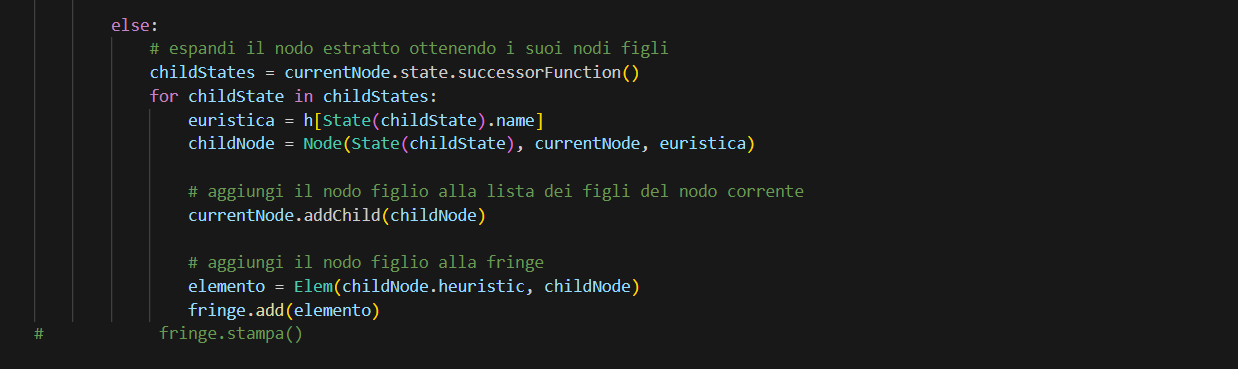
\includegraphics[width=18cm, height=7cm]{Screenshot 2024-11-10 180402.png} % Percorso dell'immagine
    %\caption{Ricerca golosa con funzione euristica h=h$_{\text{SLD}}$} % Didascalia per l'immagine
    \label{fig:immagine} % Etichetta per riferimento
\end{figure}
\subsection{L'Algoritmo A*}
Questo algoritmo ha come \textbf{Funzione di valutazione}: $f(n) = g(n) + h(n)$ ovvero la stima del costo del cammino a costo minimo dallo stato iniziale a un obiettivo, vincolato a passare per lo stato n.
\begin{figure}[H] % Usa 'H' per forzare la posizione qui
    \centering % Centra l'immagine
    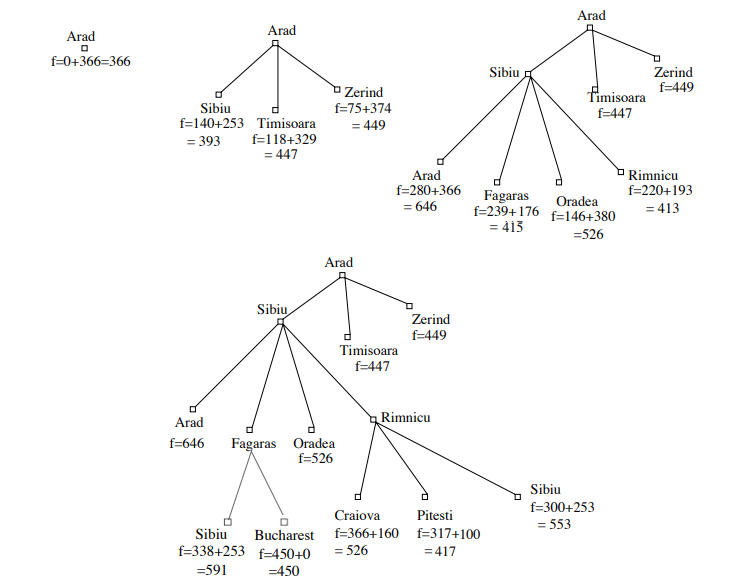
\includegraphics[width=13cm, height=8cm]{immagine_2024-11-07_174557854.png} % Percorso dell'immagine
    \caption{Visita A* (1)} % Didascalia per l'immagine
    \label{fig:immagine} % Etichetta per riferimento
\end{figure}
\noindent
g(n) rappresenta il "costo accumulato" dal nodo iniziale fino al nodo n, mentre h(n) è una stima del costo minimo per raggiungere l'obiettivo partendo da n. Volendo fare un esempio: osserviamo l'espansione del nodo Sibiu; g(Sibiu)=140: rappresenta il costo del percorso dal nodo iniziale "Arad" fino a "Sibiu". h(Sibiu)=253: rappresenta la stima del costo rimanente da "Sibiu" a "Bucharest" (quella che trovi nella tabella sopracitata).
\begin{figure}[H] % Usa 'H' per forzare la posizione qui
    \centering % Centra l'immagine
    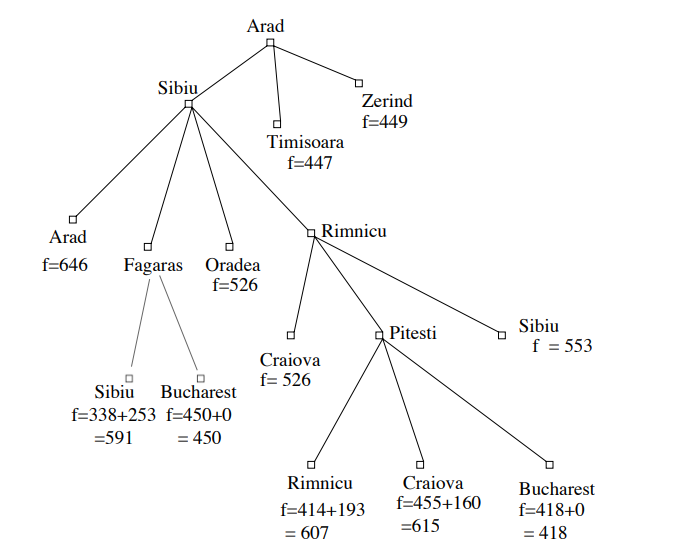
\includegraphics[width=13cm, height=8cm]{immagine_2024-11-07_174625502.png} % Percorso dell'immagine
    \caption{Visita A* (2)} % Didascalia per l'immagine
    \label{fig:immagine} % Etichetta per riferimento
\end{figure}
\subsection{Teorema di Completezza e Ottimalità per A*}
Un algoritmo di ricerca si dice completo se è garantito che troverà una soluzione (se esiste). A* è completo se:
\begin{itemize}
    \item Ogni nodo del grafo ha un numero finito di successori.
    \item Tutti gli archi hanno costi maggiori di una quantità positiva $\delta$
\end{itemize}
\begin{figure}[H] % Usa 'H' per forzare la posizione qui
    \centering % Centra l'immagine
    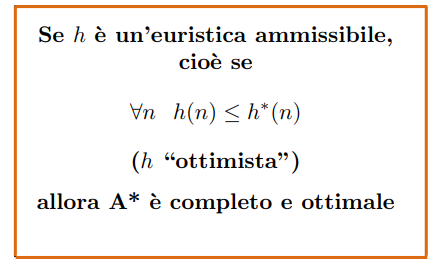
\includegraphics[width=7cm, height=4cm]{Screenshot 2024-11-07 175820.png} % Percorso dell'immagine
    %\caption{Visita A* (2)} % Didascalia per l'immagine
    \label{fig:immagine} % Etichetta per riferimento
\end{figure}
\noindent
Se due versioni di A*, che possiamo chiamare $A_1$* e $A_2$*, differiscono soltanto per il fatto che $h_1 < h_2$ per tutti i nodi non obiettivo, si dice che $A_2$* è più informato di $A_1$*.
\begin{figure}[H] % Usa 'H' per forzare la posizione qui
    \centering % Centra l'immagine
    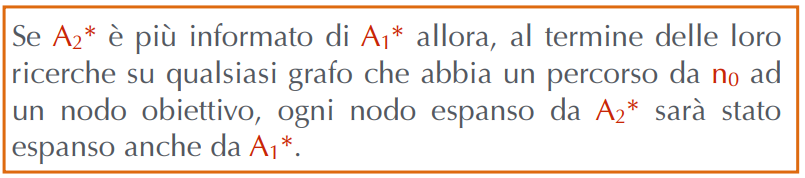
\includegraphics[width=12cm, height=3cm]{immagine_2024-11-07_181034152.png} % Percorso dell'immagine
    \caption{Influenza di H sull'efficienza} % Didascalia per l'immagine
    \label{fig:immagine} % Etichetta per riferimento
\end{figure}
\noindent
Da questo teorema segue che $A_1$* espande almeno tanti nodi quanti ne espande $A_2$*.
\subsection{Esercizio per A* (Esercizio d'esame)}
\begin{figure}[H] % Usa 'H' per forzare la posizione qui
    \centering % Centra l'immagine
    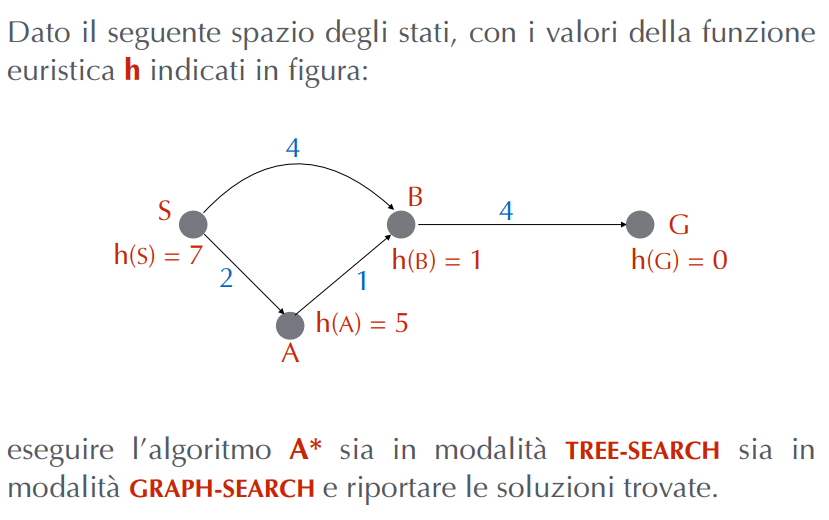
\includegraphics[width=12cm, height=8cm]{Screenshot 2024-11-07 181639.png} % Percorso dell'immagine
    %\caption{Influenza di H sull'efficienza} % Didascalia per l'immagine
    \label{fig:immagine} % Etichetta per riferimento
\end{figure}
\noindent
\begin{figure}[htbp]
    \begin{minipage}[b]{0.45\textwidth} % Prima figura a sinistra
        \centering
        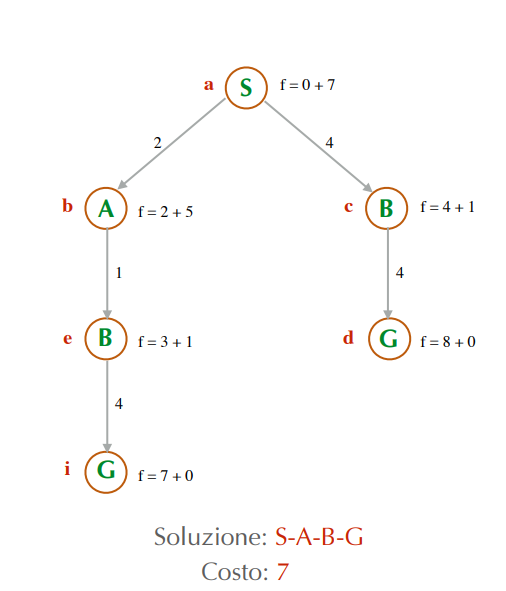
\includegraphics[width=6cm, height=7cm]{Screenshot 2024-11-07 181838.png} % Sostituisci con il nome del tuo file immagine
        \caption{Tree Search}
    \end{minipage}
    \hfill
    \begin{minipage}[b]{0.45\textwidth} % Seconda figura a destra
        \centering
        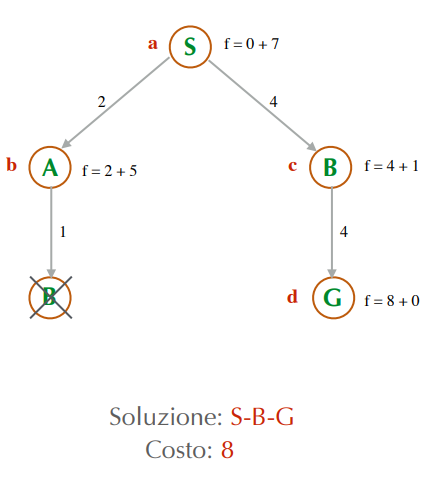
\includegraphics[width=6cm, height=7cm]{immagine_2024-11-07_182209986.png} % Sostituisci con il nome del tuo file immagine
        \caption{Graph Search}
    \end{minipage}
\end{figure}
\noindent
Vi è una differenza sostanziale nel trattamento dei nodi da parte delle due modalità:\\
\textbf{Graph Search}: tiene traccia dei nodi visitati (usando una struttura come una lista o un set) per evitare di riespandere nodi già esplorati, risparmiando tempo e riducendo i duplicati. \\
\textbf{Tree Search}: non ha un controllo sui nodi già espansi. Quindi, se un nodo è raggiungibile da più percorsi, potrebbe essere riesplorato ogni volta che viene trovato tramite un percorso differente.\\
\subsubsection{Algoritmo A* Codice Python (versione Tree Search)}

\begin{figure}[H] % Usa 'H' per forzare la posizione qui
    \centering % Centra l'immagine
    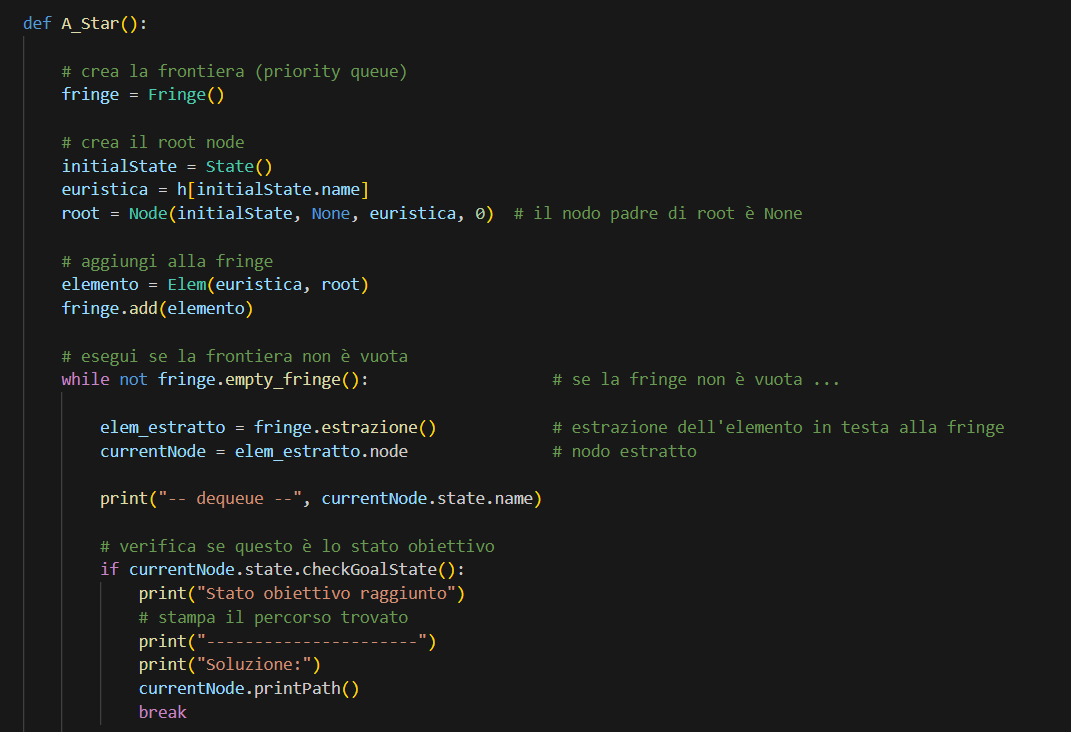
\includegraphics[width=18cm, height=10cm]{Screenshot 2024-11-10 181019.png} % Percorso dell'immagine
    %\caption{Ricerca golosa con funzione euristica h=h$_{\text{SLD}}$} % Didascalia per l'immagine
    \label{fig:immagine} % Etichetta per riferimento
\end{figure}
\begin{figure}[H] % Usa 'H' per forzare la posizione qui
    \centering % Centra l'immagine
    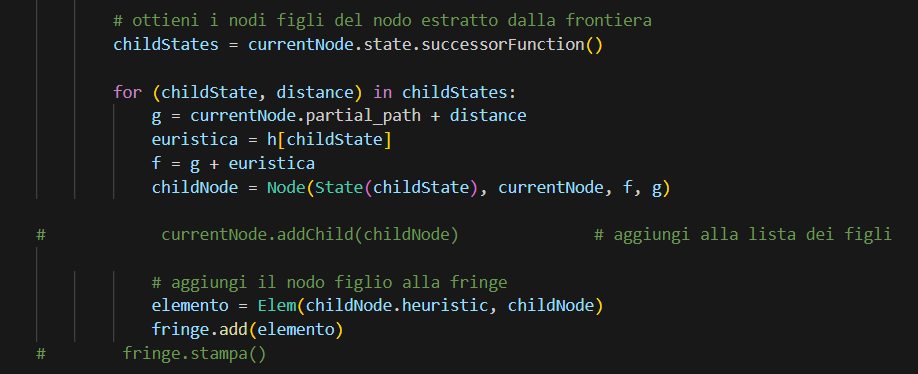
\includegraphics[width=18cm, height=7cm]{Screenshot 2024-11-10 181028.png} % Percorso dell'immagine
    %\caption{Ricerca golosa con funzione euristica h=h$_{\text{SLD}}$} % Didascalia per l'immagine
    \label{fig:immagine} % Etichetta per riferimento
\end{figure}
\subsubsection{Algoritmo A* Codice Python (versione Graph Search)}

\begin{figure}[H] % Usa 'H' per forzare la posizione qui
    \centering % Centra l'immagine
    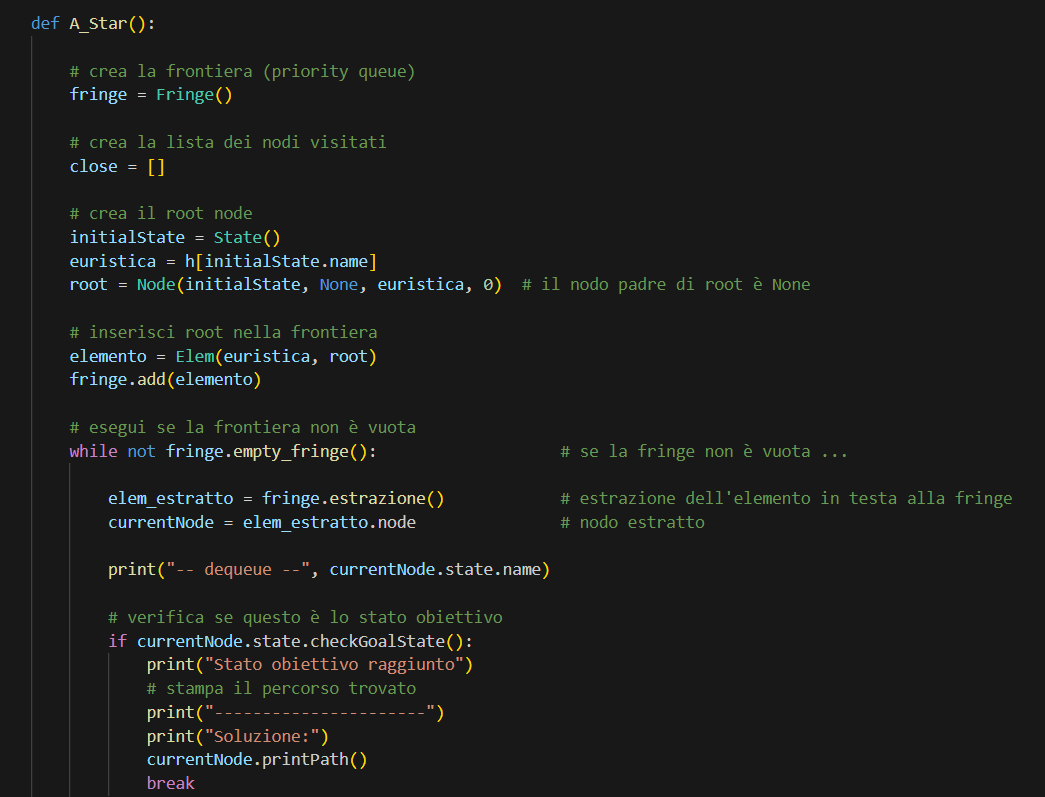
\includegraphics[width=18cm, height=10cm]{Screenshot 2024-11-10 181338.png} % Percorso dell'immagine
    %\caption{Ricerca golosa con funzione euristica h=h$_{\text{SLD}}$} % Didascalia per l'immagine
    \label{fig:immagine} % Etichetta per riferimento
\end{figure}
\begin{figure}[H] % Usa 'H' per forzare la posizione qui
    \centering % Centra l'immagine
    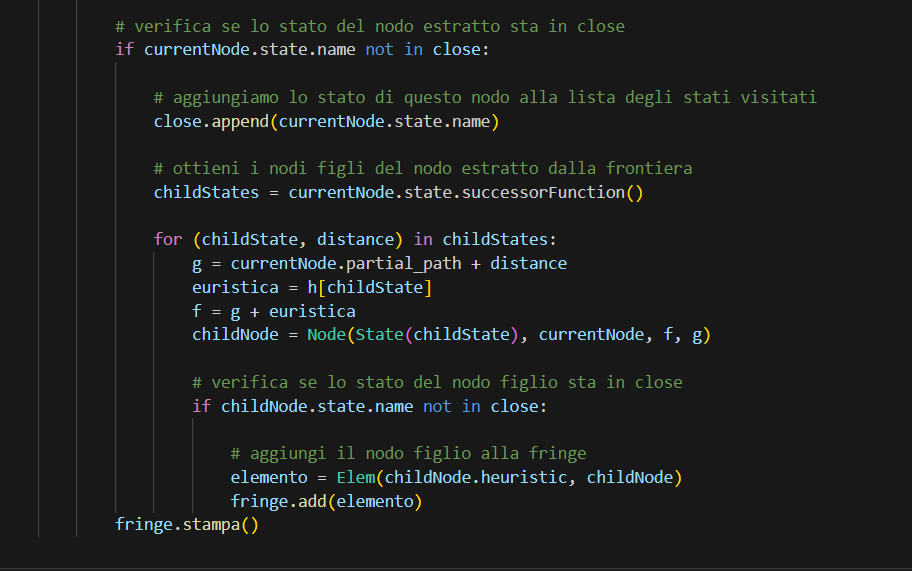
\includegraphics[width=18cm, height=7cm]{Screenshot 2024-11-10 181347.png} % Percorso dell'immagine
    %\caption{Ricerca golosa con funzione euristica h=h$_{\text{SLD}}$} % Didascalia per l'immagine
    \label{fig:immagine} % Etichetta per riferimento
\end{figure}
\vspace{80pt}
\subsection{La condizione di consistenza}
Consideriamo una coppia di nodi in cui $n_j$ è un successore di $n_i$. Diciamo che h obbedisce alla condizione di consistenza se per tutte le coppie di nodi di questo tipo nel grafo di ricerca:
$$h(n_j)\leq c(n_i,n_j) + h(n_j) $$
Dove $c(n_i,n_j)$ è il costo dell'arco da $n_i$ a $n_j$.
\begin{figure}[H] % Usa 'H' per forzare la posizione qui
    \centering % Centra l'immagine
    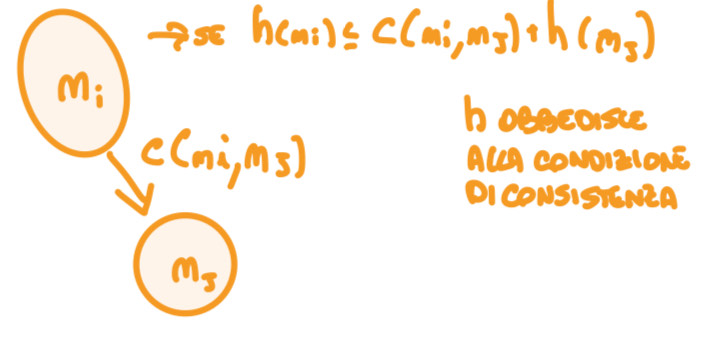
\includegraphics[width=7cm, height=3cm]{IMG_0801.jpeg} % Percorso dell'immagine
    %\caption{Influenza di H sull'efficienza} % Didascalia per l'immagine
    \label{fig:immagine} % Etichetta per riferimento
\end{figure}
\noindent
La condizione di consistenza può anche essere considerata come un tipo di diseguaglianza triangolare:
\begin{figure}[H] % Usa 'H' per forzare la posizione qui
    \centering % Centra l'immagine
    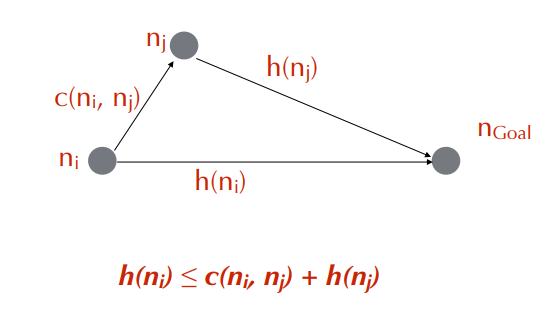
\includegraphics[width=7cm, height=4cm]{Screenshot 2024-11-09 160053.png} % Percorso dell'immagine
    %\caption{Influenza di H sull'efficienza} % Didascalia per l'immagine
    \label{fig:immagine} % Etichetta per riferimento
\end{figure}
\noindent
Dati $n_i$ e $n_j$, con $n_j$ successore di $n_i$: $$f(n_j)\geq f(n_i)$$
\subsubsection{Teorema}
\textbf{Se la condizione di consistenzxa su h è soddisfatta, allora quando A* espande un nodo n, esso ha già trovato un percorso ottimo per n}.
Infatti nel Graph Search di prima:
\begin{figure}[H] % Usa 'H' per forzare la posizione qui
    \centering % Centra l'immagine
    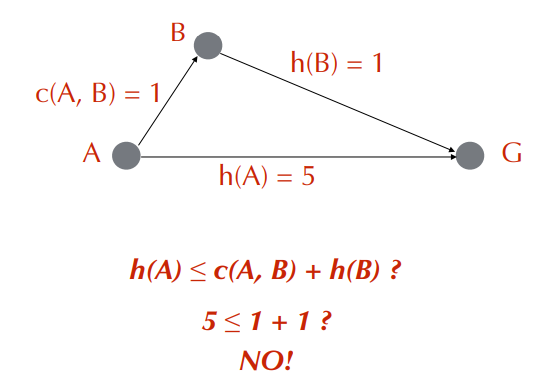
\includegraphics[width=7cm, height=4cm]{Screenshot 2024-11-09 160617.png} % Percorso dell'immagine
    %\caption{Influenza di H sull'efficienza} % Didascalia per l'immagine
    \label{fig:immagine} % Etichetta per riferimento
\end{figure}
\vspace{100pt}
\section{Local Search}
\subsection{Introduzione}
Ci sono dei problemi in cui lo stato obiettivo contiene tutte le informazioni rilevanti per la soluzione. In tali casi il cammino verso l'obiettivo è irrilevante. Gli algoritmi di ricerca locale si muovono sulla superficie cercando i picchi più alti
\begin{figure}[H] % Usa 'H' per forzare la posizione qui
    \centering % Centra l'immagine
    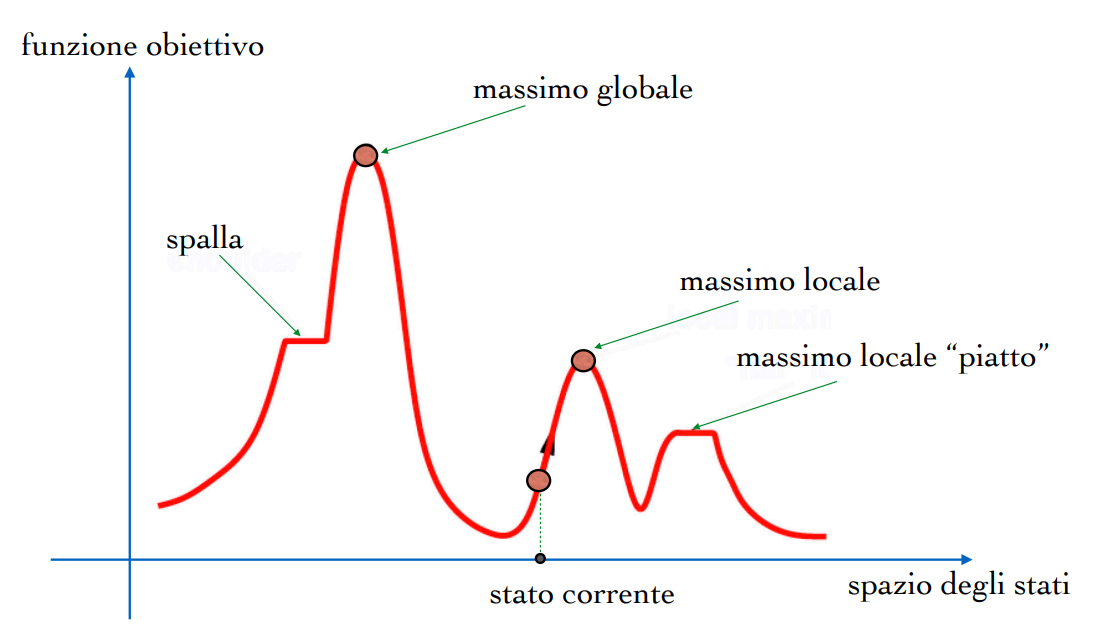
\includegraphics[width=7cm, height=4cm]{Screenshot 2024-11-10 155741.png} % Percorso dell'immagine
    %\caption{Influenza di H sull'efficienza} % Didascalia per l'immagine
    \label{fig:immagine} % Etichetta per riferimento
\end{figure}
\subsection{Hill Climbing}
Il termine \textbf{Hill Climbing} che letteralmente significa "scalatore di colline", deriva dal fatto che segue sempre le salite più rapide. Si tratta di un semplice ciclo che si muove continuamente verso l'alto, cioè nella direzione dei valori crescenti, e termina quando raggiunge un picco che non ha vicini di valore più alto.
\subsubsection{Steepest Ascent Hill Climbing}
Questo algoritmo segue le salite più ripide e può incappare in massimi locali.
\begin{figure}[H] % Usa 'H' per forzare la posizione qui
    \centering % Centra l'immagine
    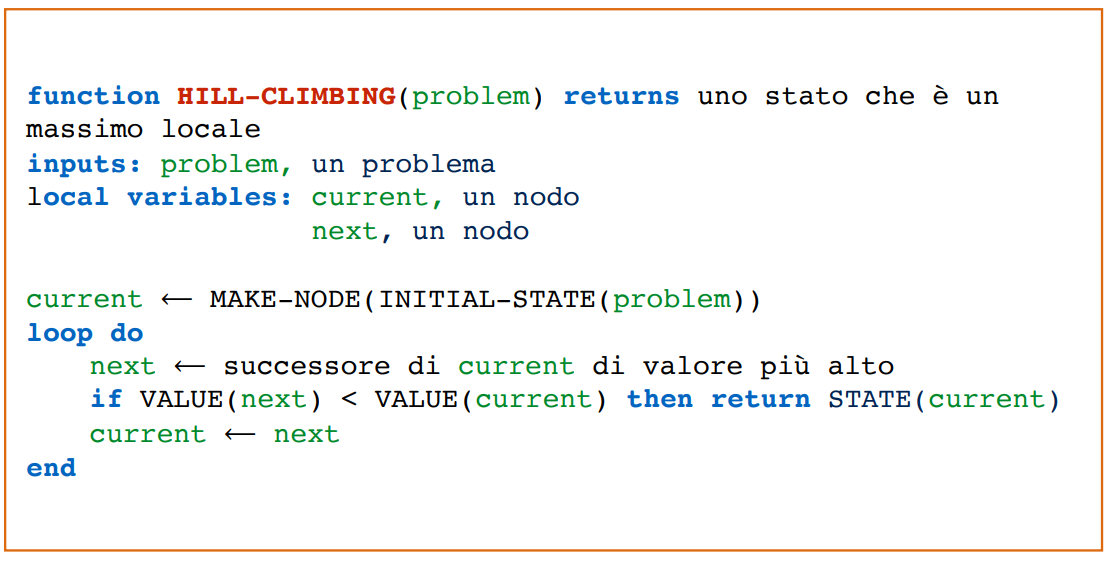
\includegraphics[width=14cm, height=6cm]{Screenshot 2024-11-10 161259.png} % Percorso dell'immagine
    \caption{Steepest Ascent} % Didascalia per l'immagine
    \label{fig:immagine} % Etichetta per riferimento
\end{figure}
\vspace{100pt}
\subsubsection{Random Restart Hill Climbing}
L'algoritmo è in un Hill-Climbing con riavvio casuale. Esso conduce una serie di ricerche Hill Climbing partendo da stati iniziali generati casualmente. L'algoritmo è completo, con probabilità tendente a 1, per la banale ragione che prima o poi dovrà generare, come stato iniziale, proprio un obiettivo.
\begin{figure}[H] % Usa 'H' per forzare la posizione qui
    \centering % Centra l'immagine
    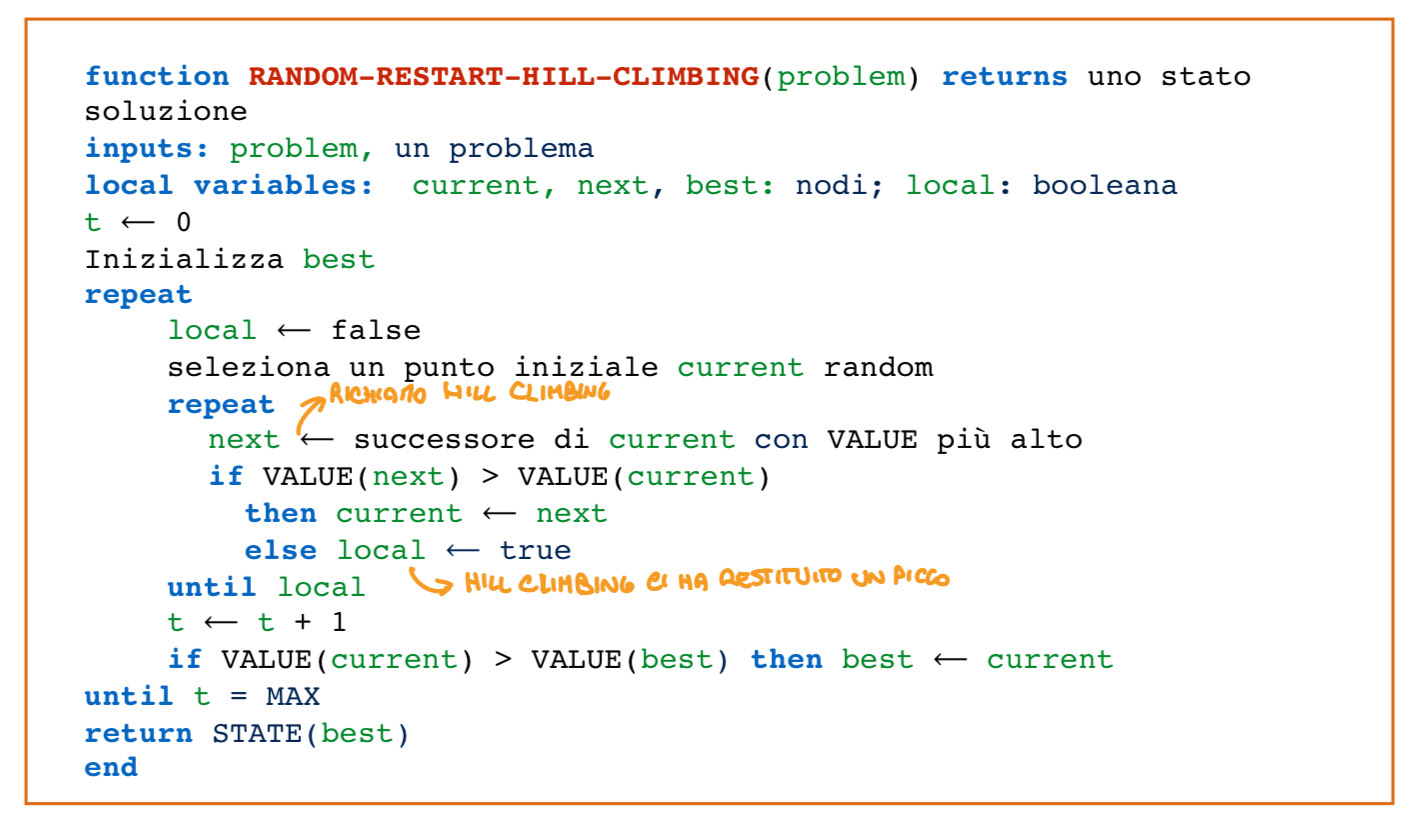
\includegraphics[width=14cm, height=7cm]{IMG_0802.jpeg} % Percorso dell'immagine
    \caption{Random Restart} % Didascalia per l'immagine
    \label{fig:immagine} % Etichetta per riferimento
\end{figure}
Il ciclo interno della procedura restituisce sempre un ottimo locale (con il numero delle scelte all'infinito trovo l'ottimo). La procedura sfugge dagli ottimi locali solo avviando una nuova ricerca partendo da un nuovo punto scelto casualmente.
\subsubsection{Stochastic Hill-Climbing}
L'algoritmo Stochastic Hill-Climbing si ottiene modificando la procedura precedente: anzichè valutare tutti i punti vicini a current e selezionare il migliore, selezioniamo casualmente solo un punto next (questo meccanismo gli permette di sfuggire dagli ottimi locali dato che potrebbe essere scelto un next peggiore). Accettiamo next con una probabilità che dipende dalla differenza di valutazione tra i due punti: $$\Delta E=VALUE(current)-VALUE(next)$$
\begin{figure}[H] % Usa 'H' per forzare la posizione qui
    \centering % Centra l'immagine
    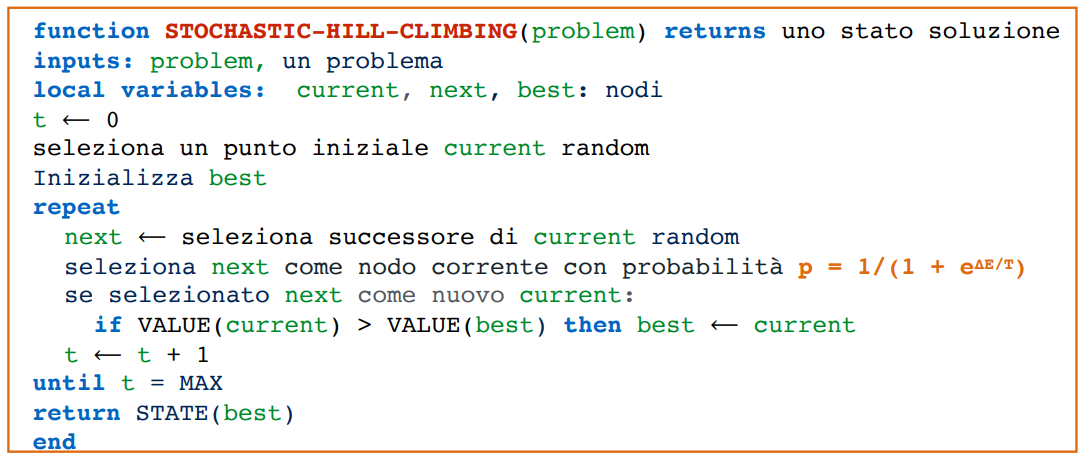
\includegraphics[width=15cm, height=6cm]{immagine_2024-11-10_162630792.png} % Percorso dell'immagine
    \caption{Stochastic Hill-Climbing} % Didascalia per l'immagine
    \label{fig:immagine} % Etichetta per riferimento
\end{figure}
\noindent
Il nuovo punto accettato viene selezionato con probabilità p. Al crescere di T diventa sempre meno importante la differenza delle valutazioni dei due punti e la probabilità di accettazione diminuisce. Al variare di next invece quello che succede è che: andare a un next peggiore è possibile ma con probabilità molto bassa, se ha lo stesso valore di current la probabilità è del 50\% mentre al crescere di next la probabilità di accettazione aumenta. Il problema risolto nell'algoritmo è relativo al passaggio dai valori di $\frac{\Delta E}{T}$ a quelli delle probabilità. $\frac{\Delta E}{T}$ ha un range che va da $-\infty$ a $+\infty$ la probabilità invece va da 0 a 1. L'espressione usata nell'algoritmo per la probabilità è in buona sostanza una "link function" che realizza un mapping tra i due intervalli:
\begin{figure}[H] % Usa 'H' per forzare la posizione qui
    \centering % Centra l'immagine
    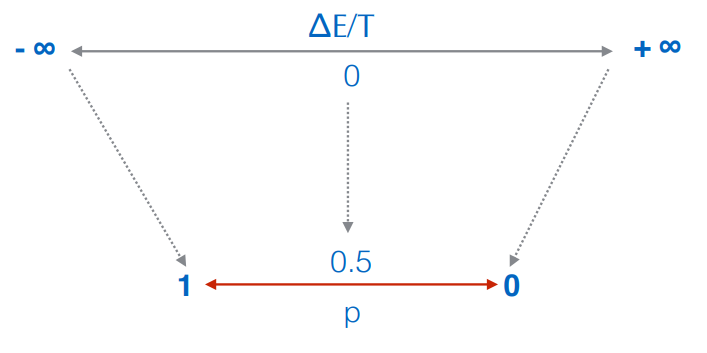
\includegraphics[width=8cm, height=5cm]{immagine_2024-11-10_163652061.png} % Percorso dell'immagine
    \caption{Link Function} % Didascalia per l'immagine
    \label{fig:immagine} % Etichetta per riferimento
\end{figure}
\subsubsection{Hill Climbing codice Python}
La versione di Hill Climbing che andremo a implementare si chiama \textbf{First-Choice Hill Climbing}. Esso, dato uno stato corrente, sceglie casualemente un successore, e passa al nuovo stato se la valutazione di tale successore è migliore di quella dello stato corrente.
\begin{figure}[H] % Usa 'H' per forzare la posizione qui
    \centering % Centra l'immagine
    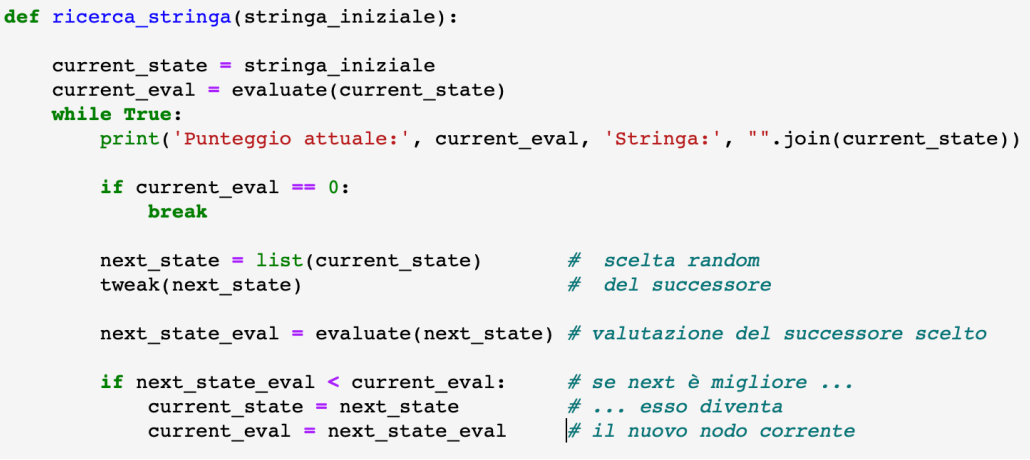
\includegraphics[width=13cm, height=6cm]{Screenshot 2024-11-10 174057.png} % Percorso dell'immagine
    %\caption{Link Function} % Didascalia per l'immagine
    \label{fig:immagine} % Etichetta per riferimento
\end{figure}
\vspace{150pt}
\subsection{Simulated Annealing}
L'algoritmo di Simulated Annealing prende il nome dall'analogia con il processo di ricottura in metallurgia che consiste nel ridurre gradualmente la temperatura di un materiale in modo da permettere alla sua struttura cristallina di raggiungere uno stato ad energia minima. È un algoritmo con miglioramenti iterativi che consente di sfuggire da ottimi locali durante la fase di search.\\
La differenza principale tra lo \textbf{stochastic hill-climber} e il \textbf{simulated annealing} è che quest'ultimo modifica il parametro \textbf{T} durante l'esecuzione.Il simulated annealing comincia con valori alti di \textbf{T} comportandosi in modo simile ad una pura \textbf{random search}. Poi decrementa gradualmente il valore di \textbf{T}. Verso
la fine dell’esecuzione i valori di \textbf{T} sono molto piccoli e
perciò l’algoritmo si comporta in modo simile ad un
normale \textbf{hill-climber}. Inoltre l'algoritmo accetta sempre nuovi punti se essi hanno una valutazione migliore del punto corrente.
\begin{figure}[H] % Usa 'H' per forzare la posizione qui
    \centering % Centra l'immagine
    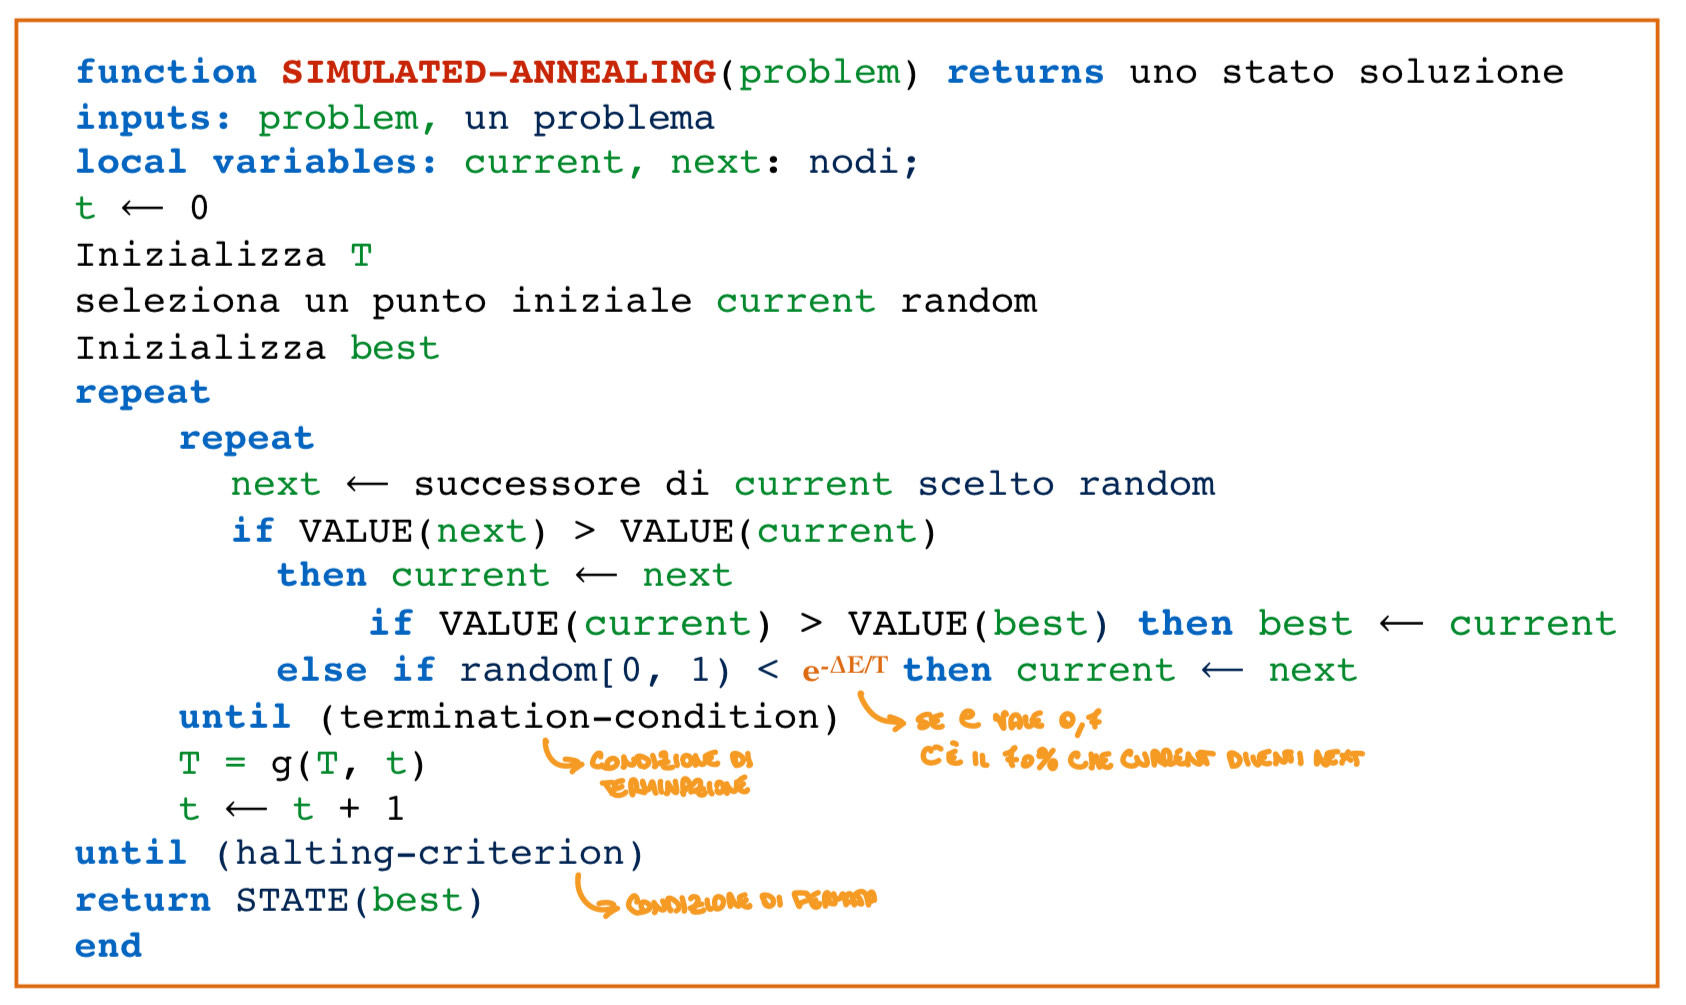
\includegraphics[width=14cm, height=7cm]{IMG_0803.jpeg} % Percorso dell'immagine
    \caption{Simulated Annealing} % Didascalia per l'immagine
    \label{fig:immagine} % Etichetta per riferimento
\end{figure}
\subsubsection{Simulated Annealing codice Python}
\textbf{La funzione Tweak}:
 Viene utilizzata per scegliere random uno stato successore.
\textbf{La funzione inizializza}:
 Serve per scegliere casualmente lo stato di partenza.
\textbf{La funzione energia}:
 È la funzione di valutazione
\begin{figure}[H] % Usa 'H' per forzare la posizione qui
    \centering % Centra l'immagine
    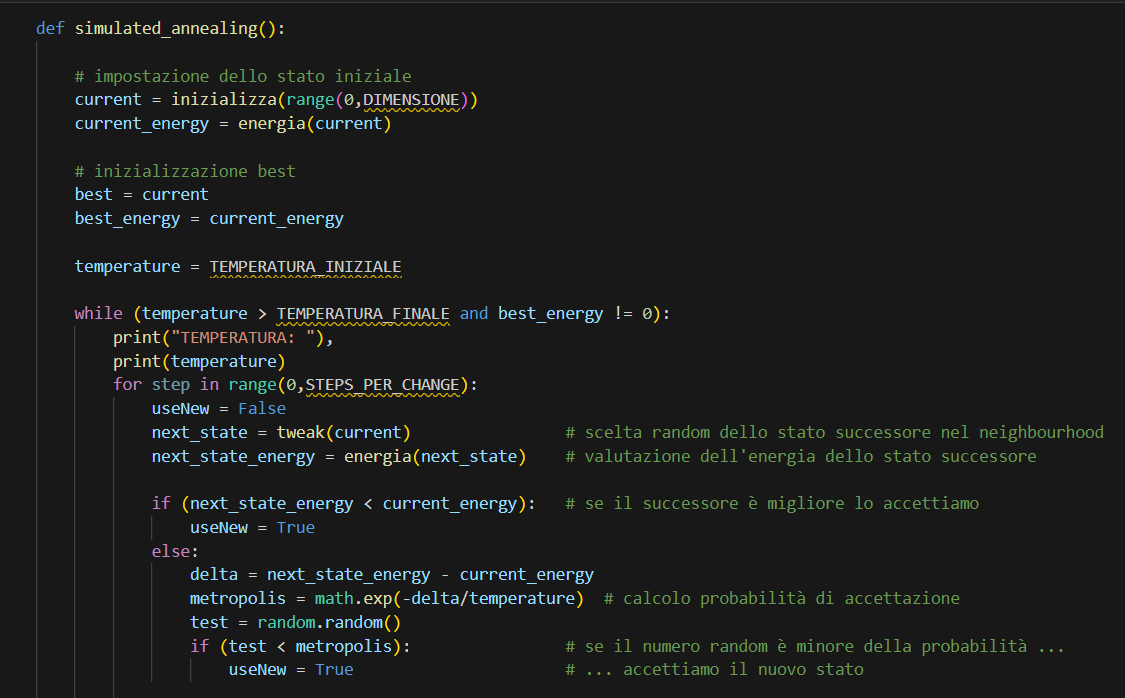
\includegraphics[width=15cm, height=7cm]{Screenshot 2024-11-10 170721.png} % Percorso dell'immagine
    %\caption{Link Function} % Didascalia per l'immagine
    \label{fig:immagine} % Etichetta per riferimento
\end{figure}
\begin{figure}[H] % Usa 'H' per forzare la posizione qui
    \centering % Centra l'immagine
    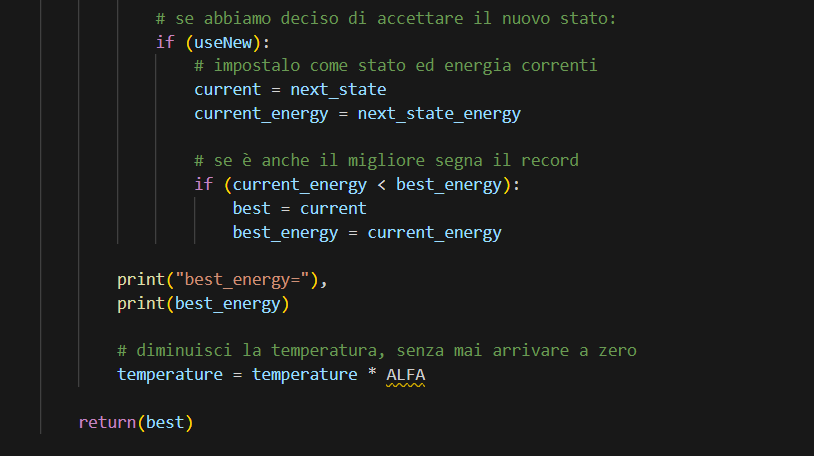
\includegraphics[width=15cm, height=7cm]{Screenshot 2024-11-10 170729.png} % Percorso dell'immagine
    %\caption{Link Function} % Didascalia per l'immagine
    \label{fig:immagine} % Etichetta per riferimento
\end{figure}
\noindent
\section{Strutture Dati in Python}
\subsection{Liste Concatenate}
\subsubsection{Liste singolarmente concatenate}
Una lista contiene dei nodi che hanno dai dati e un puntatore al nodo successivo.
\begin{figure}[H] % Usa 'H' per forzare la posizione qui
    \centering % Centra l'immagine
    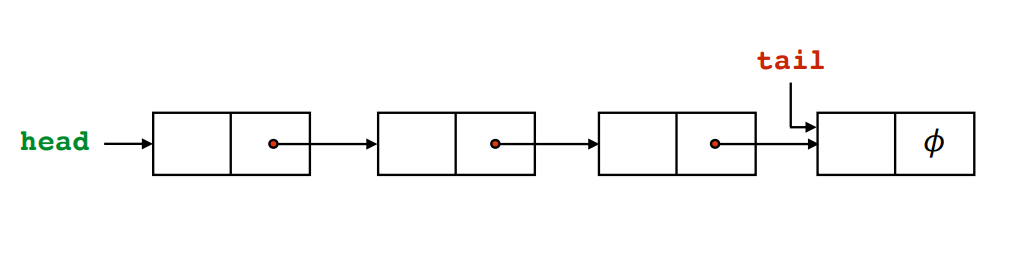
\includegraphics[width=12cm, height=4cm]{immagine_2024-11-11_160658837.png} % Percorso dell'immagine
    \caption{Rappresentazione grafica lista} % Didascalia per l'immagine
    \label{fig:immagine} % Etichetta per riferimento
\end{figure}
\noindent
\vspace{-10pt}
\textbf{Definizione della classe nodo:}\\
\begin{figure}[H] % Usa 'H' per forzare la posizione qui
    \centering % Centra l'immagine
    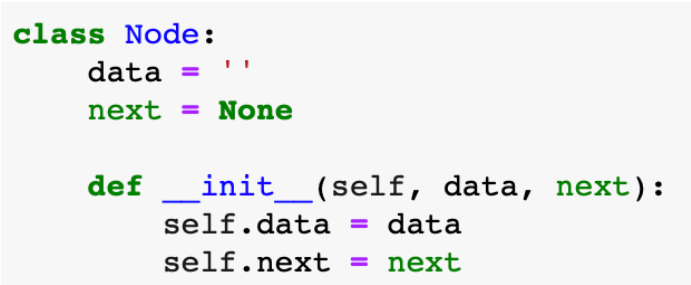
\includegraphics[width=10cm, height=4cm]{Screenshot 2024-11-11 160912.png} % Percorso dell'immagine
    \caption{Classe Nodo} % Didascalia per l'immagine
    \label{fig:immagine} % Etichetta per riferimento
\end{figure}
\noindent
\textbf{Definizione della classe lista:} (inizializzata a lista vuota)\\
\begin{figure}[H] % Usa 'H' per forzare la posizione qui
    \centering % Centra l'immagine
    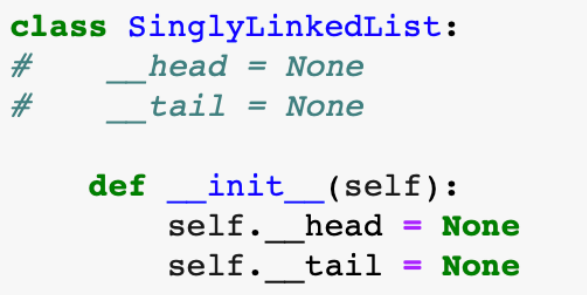
\includegraphics[width=10cm, height=4cm]{immagine_2024-11-11_161313587.png} % Percorso dell'immagine
    \caption{Classe lista} % Didascalia per l'immagine
    \label{fig:immagine} % Etichetta per riferimento
\end{figure}
\noindent
Per \textbf{scansionare la lista} bisogna partire impostando un puntatore alla testa
\begin{lstlisting}[language=Python, frame=single, numbers=left]
p = self.__head
\end{lstlisting}
\noindent
e si procede fino a raggiungere l'ultimo elemento della lista
\begin{lstlisting}[language=Python, frame=single, numbers=left]
p = p.next
\end{lstlisting}
ovvero quando p.next=None \\
\textbf{Definizione della funzione stampa\_lista} (end=' ' serve a non andare a capo alla fine della stampa, ma a lasciare uno spazio)
\begin{figure}[H] % Usa 'H' per forzare la posizione qui
    \centering % Centra l'immagine
    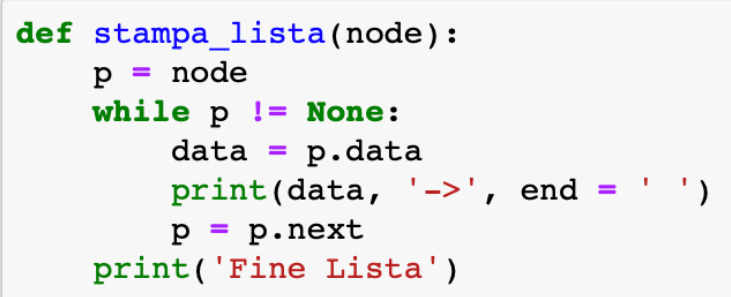
\includegraphics[width=10cm, height=4cm]{immagine_2024-11-11_162105350.png} % Percorso dell'immagine
    \caption{Funzione stampa\_lista} % Didascalia per l'immagine
    \label{fig:immagine} % Etichetta per riferimento
\end{figure}
\noindent
\textbf{Inserimento in coda (APPEND):}
\begin{figure}[H]
    \begin{minipage}[b]{0.45\textwidth} % Prima figura a sinistra
        \centering
        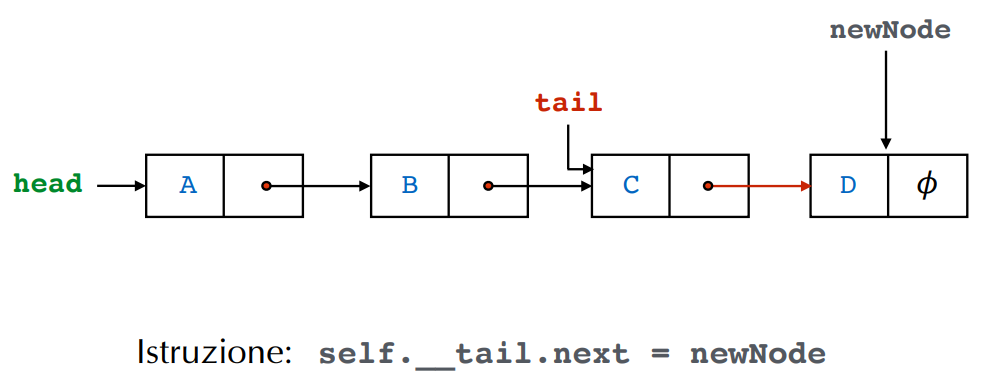
\includegraphics[width=8cm, height=5cm]{Screenshot 2024-11-11 162746.png} % Sostituisci con il nome del tuo file immagine
       % \caption{Tree Search}
    \end{minipage}
    \hfill
    \begin{minipage}[b]{0.45\textwidth} % Seconda figura a destra
        \centering
        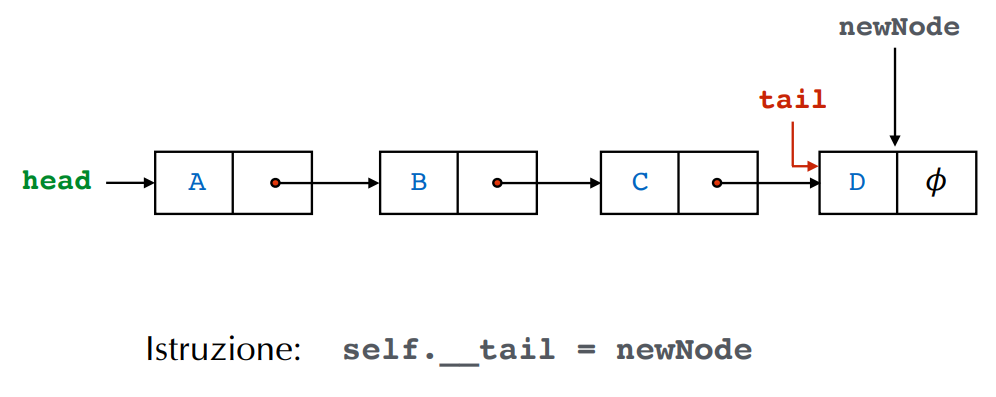
\includegraphics[width=8cm, height=5cm]{Screenshot 2024-11-11 162758.png} % Sostituisci con il nome del tuo file immagine
       % \caption{Graph Search}
    \end{minipage}
\end{figure}
\begin{lstlisting}[language=Python, frame=single, numbers=left]
self.__tail=newNode
self.__head=newNode
\end{lstlisting}
\noindent
In caso la lista fosse vuota si impostano i puntatori di testa e coda al nuovo nodo.
\begin{figure}[H] % Usa 'H' per forzare la posizione qui
    \centering % Centra l'immagine
    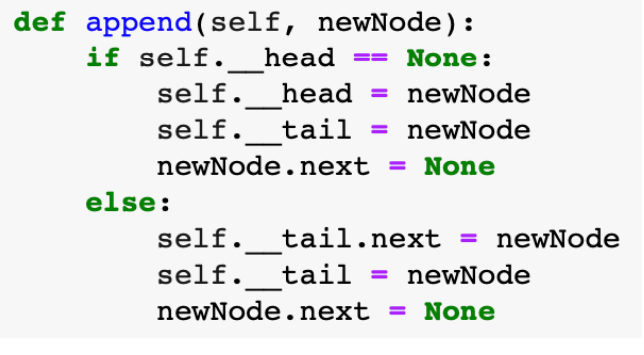
\includegraphics[width=10cm, height=4cm]{Screenshot 2024-11-11 163437.png} % Percorso dell'immagine
    \caption{Inserimento in coda} % Didascalia per l'immagine
    \label{fig:immagine} % Etichetta per riferimento
\end{figure}
\noindent
\textbf{Inserimento in testa}
\begin{figure}[H]
    \begin{minipage}[b]{0.45\textwidth} % Prima figura a sinistra
        \centering
        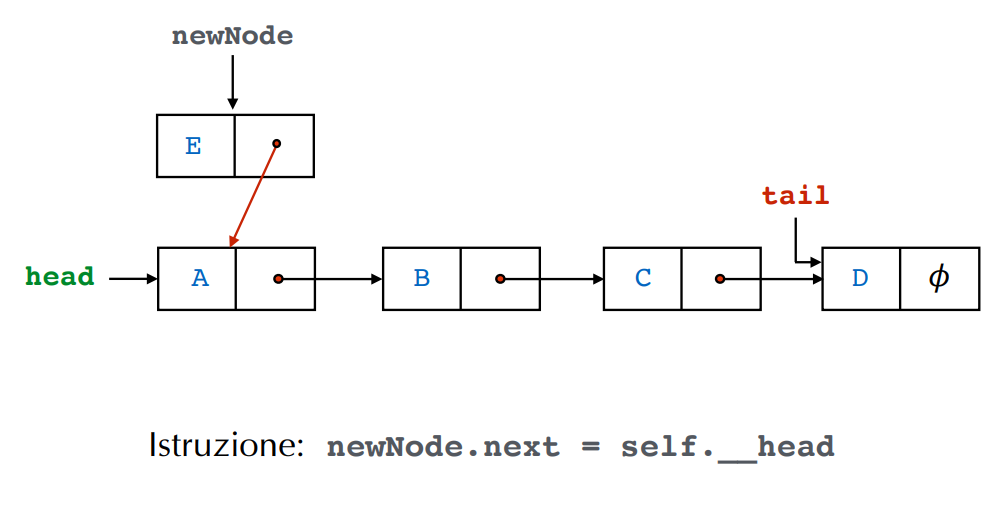
\includegraphics[width=8cm, height=5cm]{Screenshot 2024-11-11 163802.png} % Sostituisci con il nome del tuo file immagine
       % \caption{Tree Search}
    \end{minipage}
    \hfill
    \begin{minipage}[b]{0.45\textwidth} % Seconda figura a destra
        \centering
        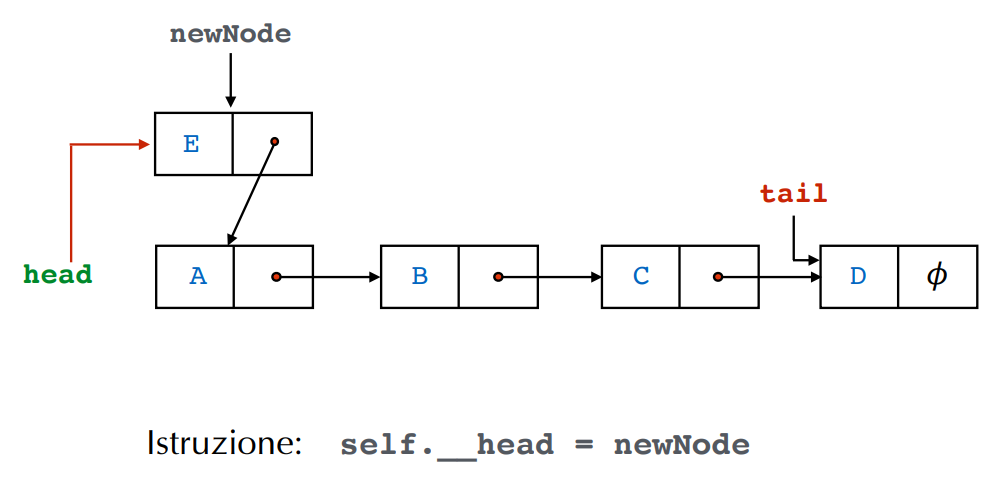
\includegraphics[width=8cm, height=5cm]{Screenshot 2024-11-11 163811.png} % Sostituisci con il nome del tuo file immagine
       % \caption{Graph Search}
    \end{minipage}
\end{figure}
Se la lista fosse vuota si procederebbe come per l'append.
\begin{figure}[H] % Usa 'H' per forzare la posizione qui
    \centering % Centra l'immagine
    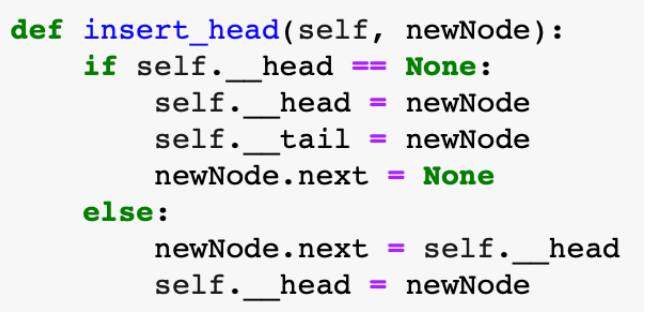
\includegraphics[width=10cm, height=4cm]{Screenshot 2024-11-11 163938.png} % Percorso dell'immagine
    \caption{Inserimento in testa} % Didascalia per l'immagine
    \label{fig:immagine} % Etichetta per riferimento
\end{figure}

\vspace{200pt}
\noindent
\textbf{Inserimento di un elemento in posizione intermedia}\\
Supponiamo di creare un nuovo nodo e di volerlo mettere in posizione i=2 (i parte da 0). Si procede fino a raggiungere la posizione precedente quella dell'inserimento (ovviamente il puntatore parte da self.\_\_head).
\begin{figure}[H]
    \begin{minipage}[b]{0.45\textwidth} % Prima figura a sinistra
        \centering
        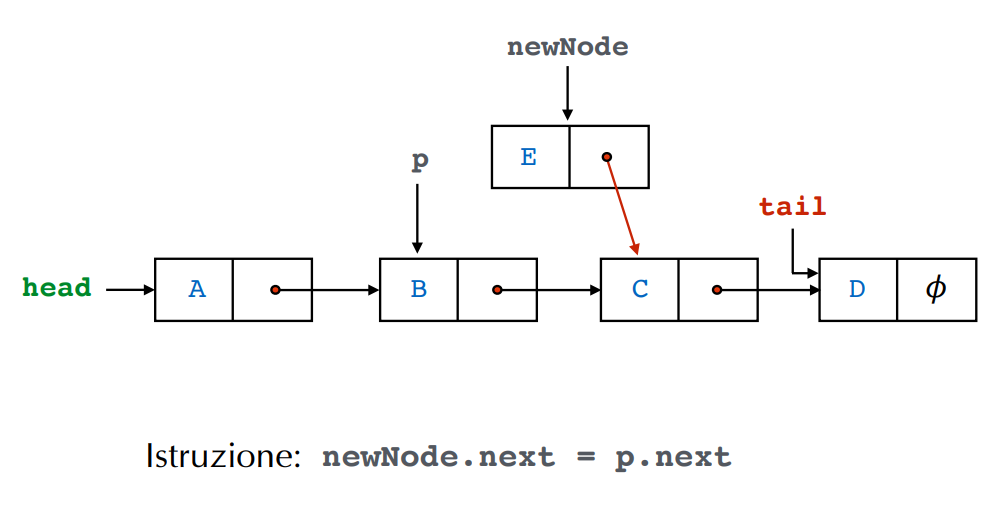
\includegraphics[width=8cm, height=5cm]{Screenshot 2024-11-11 164301.png} % Sostituisci con il nome del tuo file immagine
       % \caption{Tree Search}
    \end{minipage}
    \hfill
    \begin{minipage}[b]{0.45\textwidth} % Seconda figura a destra
        \centering
        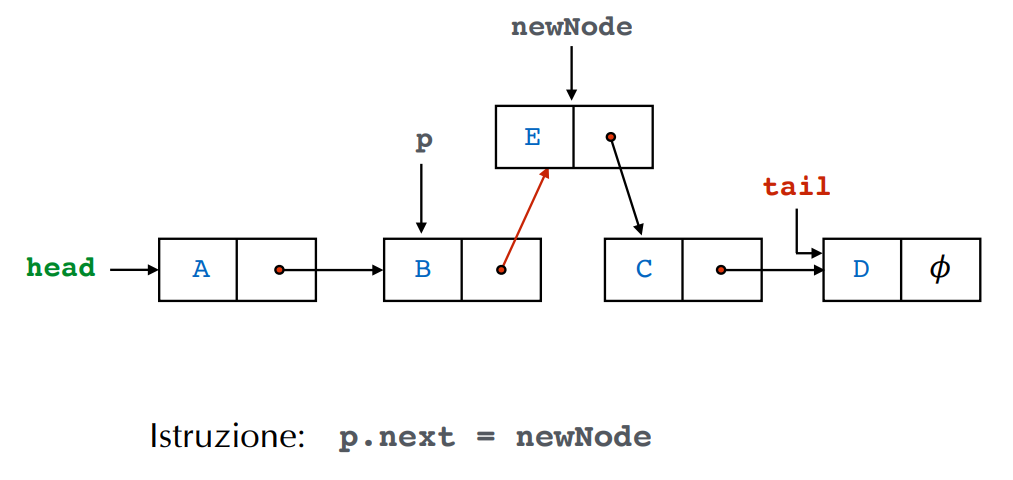
\includegraphics[width=8cm, height=5cm]{Screenshot 2024-11-11 164309.png} % Sostituisci con il nome del tuo file immagine
       % \caption{Graph Search}
    \end{minipage}
\end{figure}
\begin{figure}[H] % Usa 'H' per forzare la posizione qui
    \centering % Centra l'immagine
    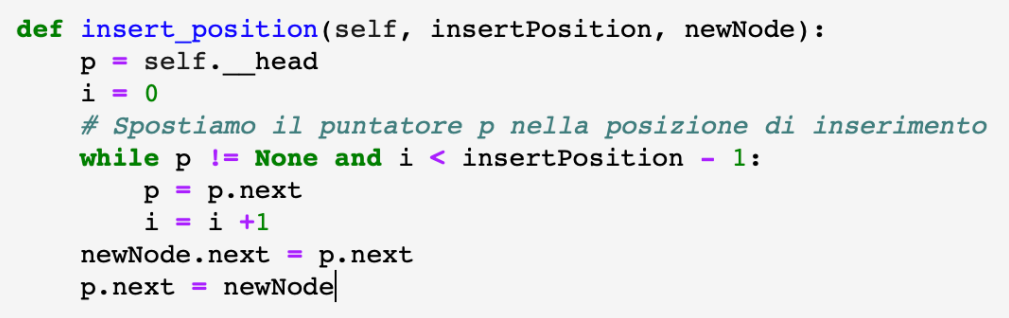
\includegraphics[width=13cm, height=4cm]{Screenshot 2024-11-11 164516.png} % Percorso dell'immagine
    \caption{Inserimento di un elemento in posizione intermedia} % Didascalia per l'immagine
    \label{fig:immagine} % Etichetta per riferimento
\end{figure}
\noindent
\textbf{Cancellazione dell'elemento i-esimo}\\
Come per l'inserimento si procede fino a raggiungere la posizione precedente a quella della cancellazione.
\begin{figure}[H]
    \begin{minipage}[b]{0.45\textwidth} % Prima figura a sinistra
        \centering
        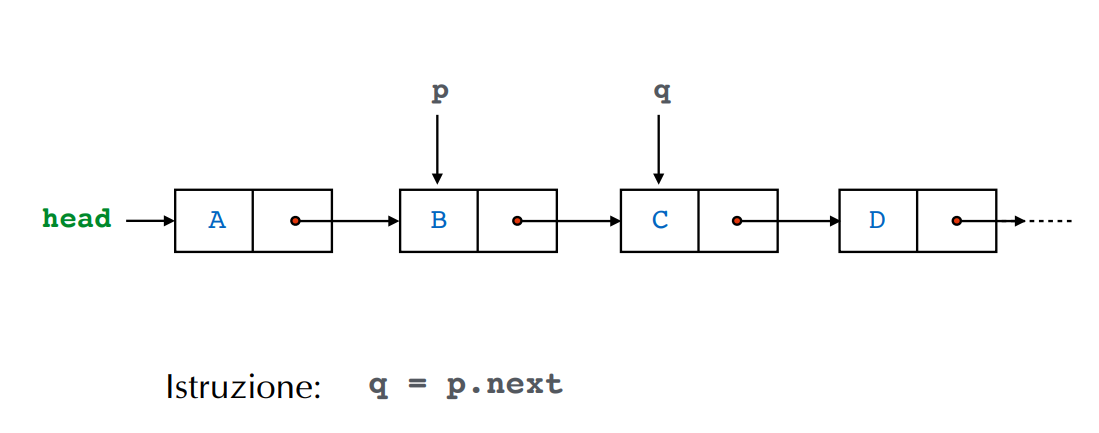
\includegraphics[width=8cm, height=5cm]{Screenshot 2024-11-11 165038.png} % Sostituisci con il nome del tuo file immagine
       % \caption{Tree Search}
    \end{minipage}
    \hfill
    \begin{minipage}[b]{0.45\textwidth} % Seconda figura a destra
        \centering
        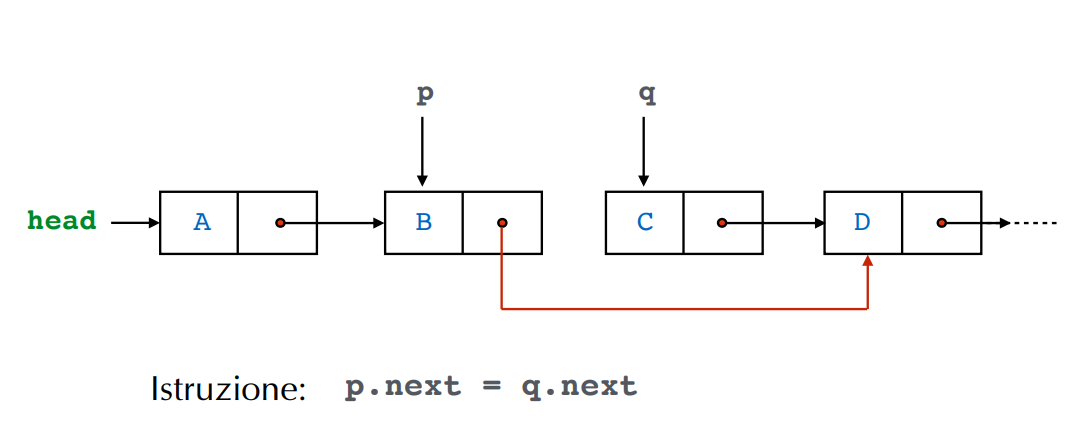
\includegraphics[width=8cm, height=5cm]{Screenshot 2024-11-11 165047.png} % Sostituisci con il nome del tuo file immagine
       % \caption{Graph Search}
    \end{minipage}
\end{figure}
\begin{figure}[H] % Usa 'H' per forzare la posizione qui
    \centering % Centra l'immagine
    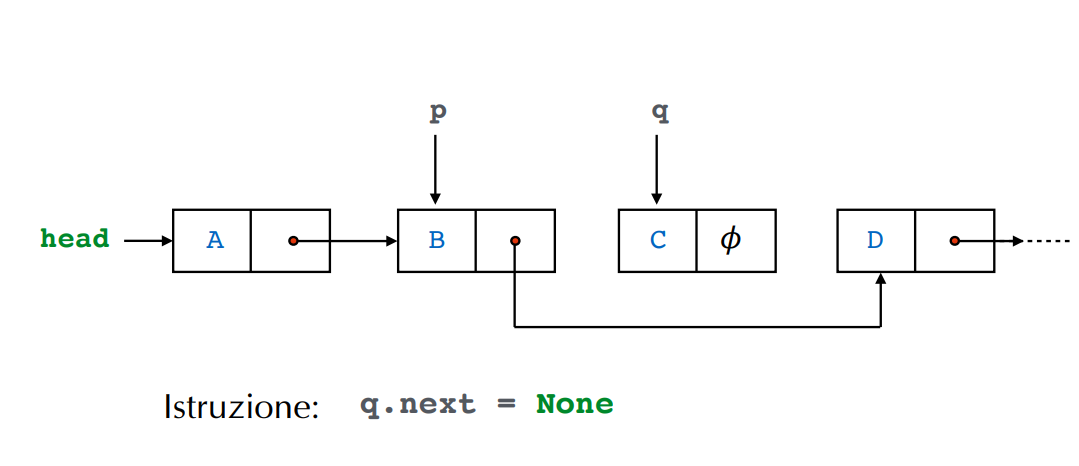
\includegraphics[width=10cm, height=5cm]{Screenshot 2024-11-11 165054.png} % Percorso dell'immagine
    %\caption{Inserimento di un elemento in posizione intermedia} % Didascalia per l'immagine
    \label{fig:immagine} % Etichetta per riferimento
\end{figure}
\begin{figure}[H] % Usa 'H' per forzare la posizione qui
    \centering % Centra l'immagine
    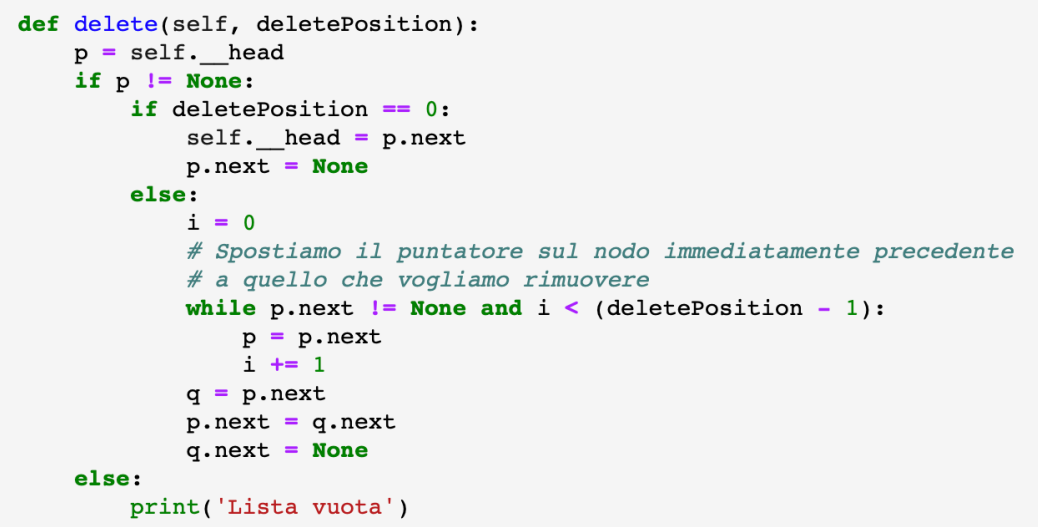
\includegraphics[width=13cm, height=6cm]{immagine_2024-11-11_165408143.png} % Percorso dell'immagine
    \caption{Cancellazione dell'elemento i-esimo} % Didascalia per l'immagine
    \label{fig:immagine} % Etichetta per riferimento
\end{figure}
\subsection{Liste Ordinate}
Una lista ordinata è una lista i cui elementi sono ordinati secondo una certa chiave. Ogni operazione di inserimento di un nuovo elemento deve dunque rispettare l'ordinamento suddetto.\\
\textbf{Definizione della classe Nodo}
\begin{figure}[H] % Usa 'H' per forzare la posizione qui
    \centering % Centra l'immagine
    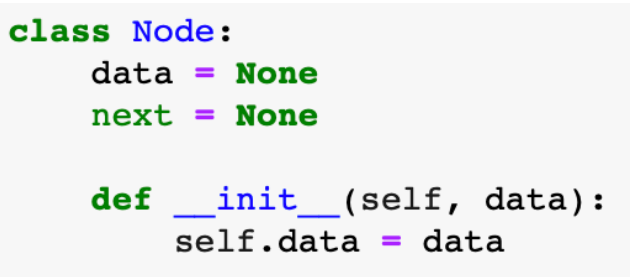
\includegraphics[width=10cm, height=5cm]{immagine_2024-11-11_173019332.png} % Percorso dell'immagine
    \caption{Definizione della classe nodo} % Didascalia per l'immagine
    \label{fig:immagine} % Etichetta per riferimento
\end{figure}
\vspace{100pt}
\noindent
\textbf{Definizione della classe lista}
\begin{figure}[H] % Usa 'H' per forzare la posizione qui
    \centering % Centra l'immagine
    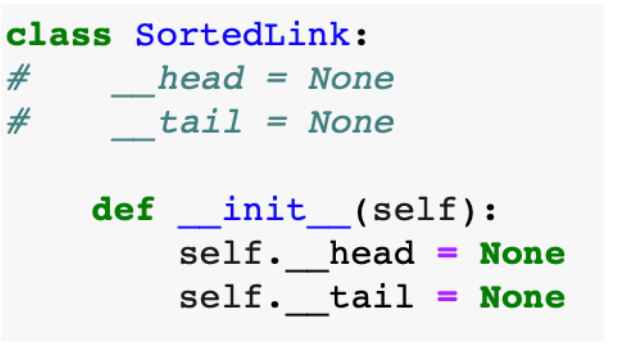
\includegraphics[width=10cm, height=5cm]{immagine_2024-11-11_173223665.png} % Percorso dell'immagine
    \caption{Definizione della classe nodo} % Didascalia per l'immagine
    \label{fig:immagine} % Etichetta per riferimento
\end{figure}
\noindent
\textbf{Inserimento in posizione intermedia}
\begin{figure}[H]
    \begin{minipage}[b]{0.45\textwidth} % Prima figura a sinistra
        \centering
        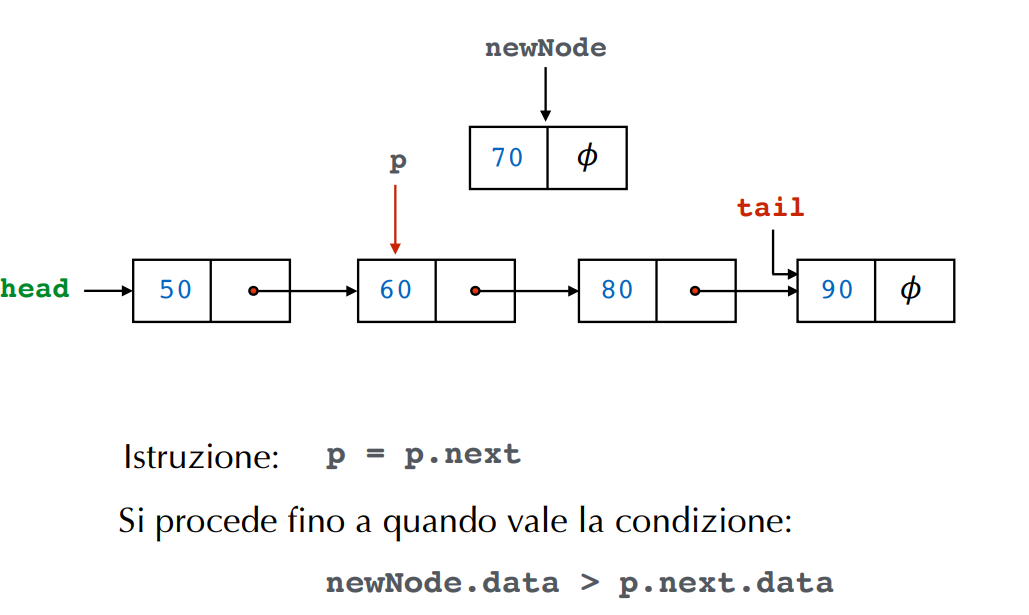
\includegraphics[width=8cm, height=5cm]{Screenshot 2024-11-11 173437.png} % Sostituisci con il nome del tuo file immagine
       % \caption{Tree Search}
    \end{minipage}
    \hfill
    \begin{minipage}[b]{0.45\textwidth} % Seconda figura a destra
        \centering
        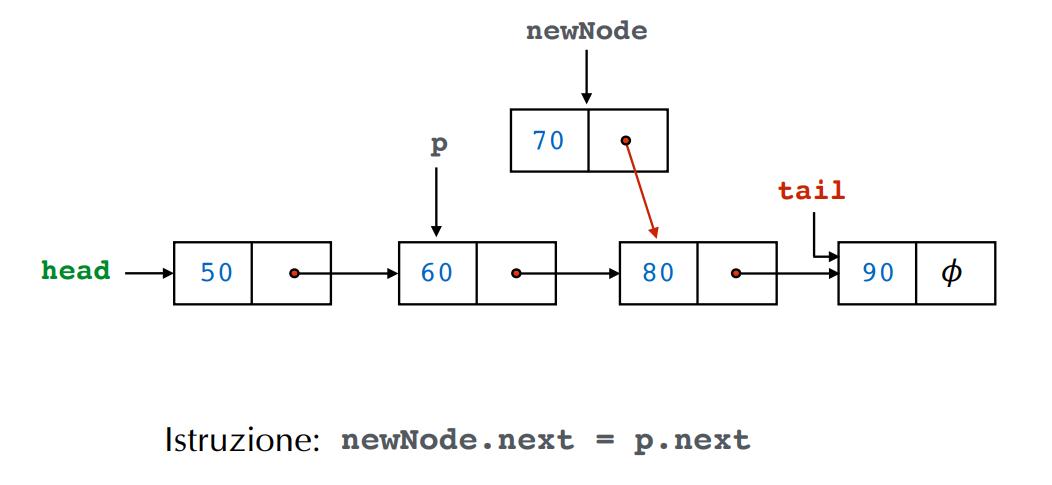
\includegraphics[width=8cm, height=5cm]{Screenshot 2024-11-11 173454.png} % Sostituisci con il nome del tuo file immagine
       % \caption{Graph Search}
    \end{minipage}
\end{figure}
\begin{figure}[H] % Usa 'H' per forzare la posizione qui
    \centering % Centra l'immagine
    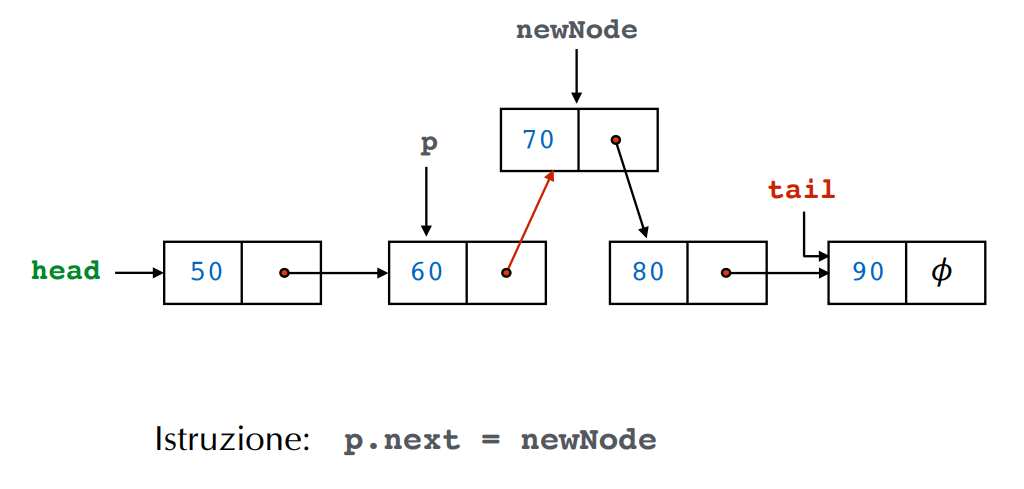
\includegraphics[width=10cm, height=4cm]{Screenshot 2024-11-11 173502.png} % Percorso dell'immagine
    \caption{Inserimento in posizione intermedia} % Didascalia per l'immagine
    \label{fig:immagine} % Etichetta per riferimento
\end{figure}
\vspace{150pt}
ovviamente c'è da considerare anche il caso in cui il valore del nodo si trovi prima dell'inizio della lista.
\begin{figure}[H]
    \begin{minipage}[b]{0.45\textwidth} % Prima figura a sinistra
        \centering
        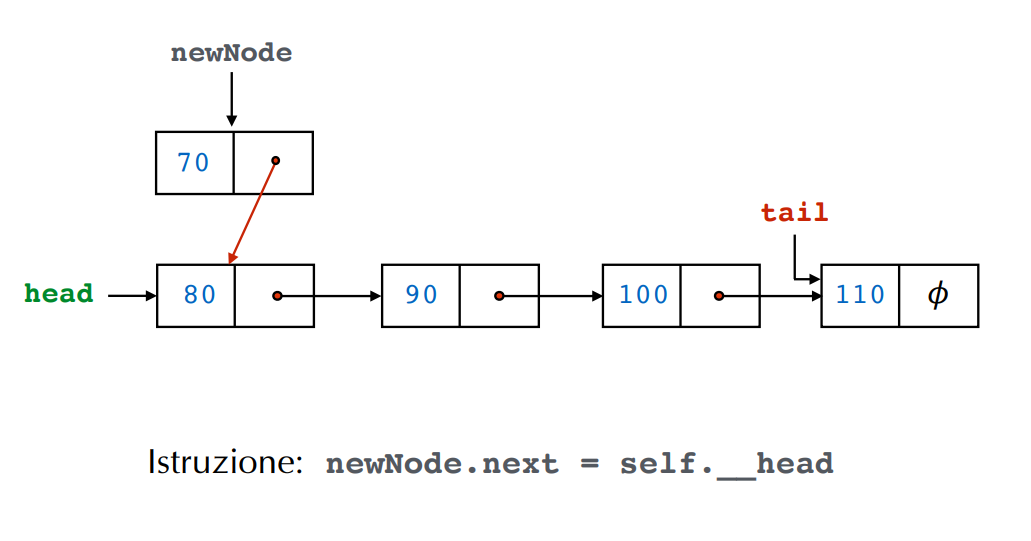
\includegraphics[width=8cm, height=5cm]{Screenshot 2024-11-11 174059.png} % Sostituisci con il nome del tuo file immagine
       % \caption{Tree Search}
    \end{minipage}
    \hfill
    \begin{minipage}[b]{0.45\textwidth} % Seconda figura a destra
        \centering
        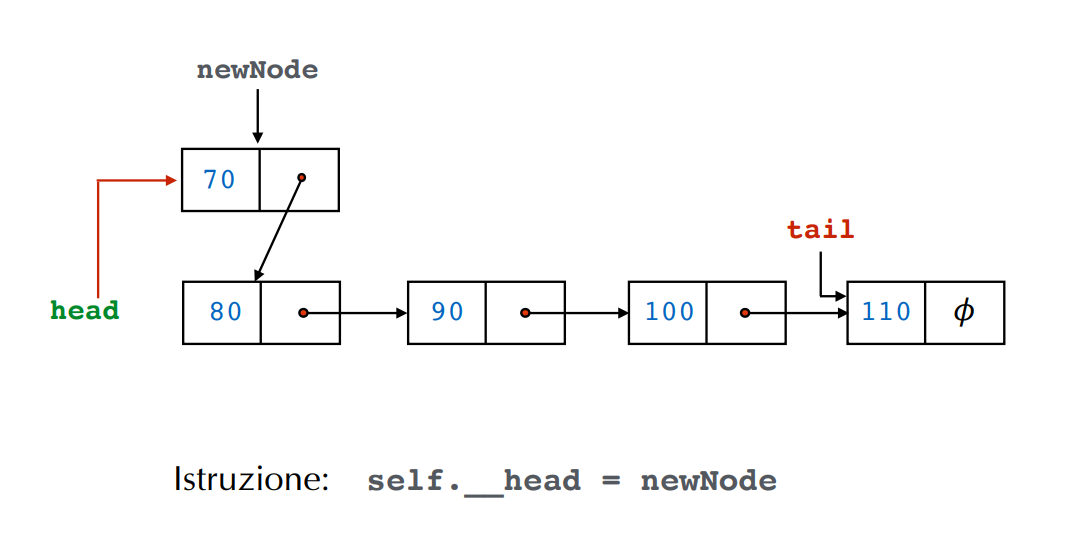
\includegraphics[width=8cm, height=5cm]{Screenshot 2024-11-11 174107.png} % Sostituisci con il nome del tuo file immagine
       % \caption{Graph Search}
    \end{minipage}
\end{figure}
In caso di lista vuota il procedimento di inserimento è quello di una lista singolarmente concatenata.
\begin{figure}[H] % Usa 'H' per forzare la posizione qui
    \centering % Centra l'immagine
    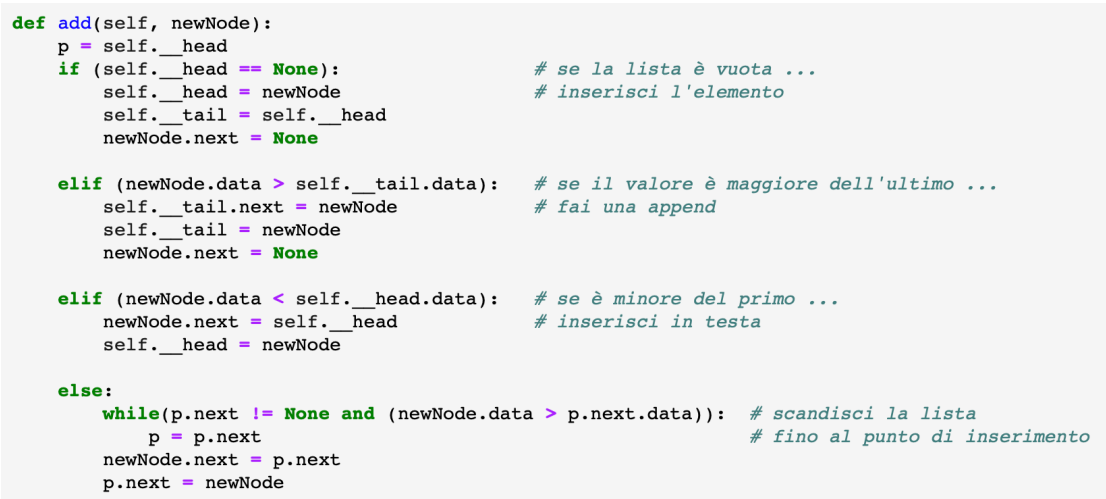
\includegraphics[width=12cm, height=6cm]{Screenshot 2024-11-11 174328.png} % Percorso dell'immagine
    \caption{Inserimento di un elemento} % Didascalia per l'immagine
    \label{fig:immagine} % Etichetta per riferimento
\end{figure}
\subsection{Le pile}
Una pila è un tipo di dato astratto, basato sul modello dei dati delle liste, in cui tutte le operazioni vengono effettuate a un estremo della lista, chiamato la \textbf{testa (top)}. La politica di gestione è la \textbf{Last-In-First-Out (LIFO)}.\\
\textbf{Definizione della classe nodo}:

\begin{figure}[H] % Usa 'H' per forzare la posizione qui
    \centering % Centra l'immagine
    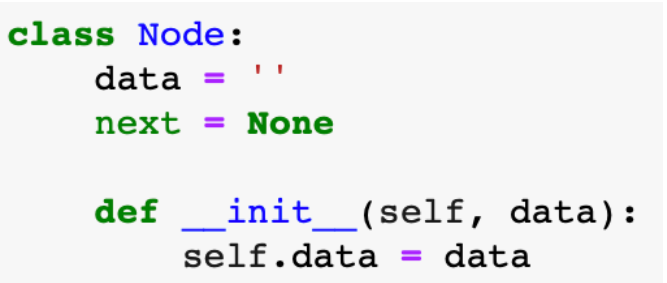
\includegraphics[width=10cm, height=5cm]{Screenshot 2024-11-11 174839.png} % Percorso dell'immagine
    \caption{Definizione della classe nodo} % Didascalia per l'immagine
    \label{fig:immagine} % Etichetta per riferimento
\end{figure}
\textbf{Definizione della classe Stack (pila)}
\begin{figure}[H] % Usa 'H' per forzare la posizione qui
    \centering % Centra l'immagine
    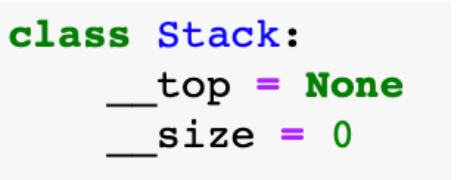
\includegraphics[width=8cm, height=3cm]{Screenshot 2024-11-11 175123.png} % Percorso dell'immagine
    \caption{Definizione della classe Stack} % Didascalia per l'immagine
    \label{fig:immagine} % Etichetta per riferimento
\end{figure}
\noindent
\textbf{Inserimento di un elemento (PUSH)}
\begin{figure}[H]
    \begin{minipage}[b]{0.45\textwidth} % Prima figura a sinistra
        \centering
        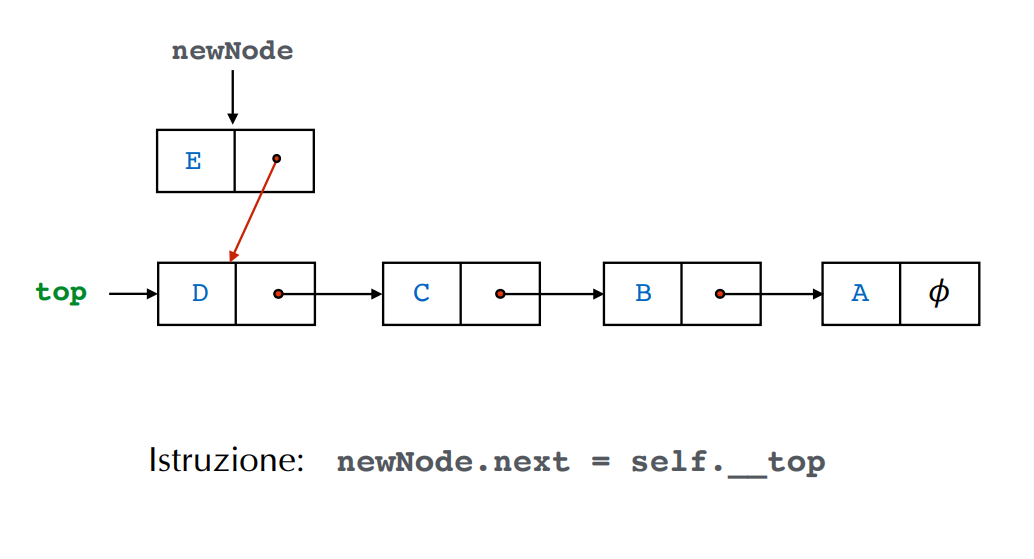
\includegraphics[width=8cm, height=5cm]{Screenshot 2024-11-11 175330.png} % Sostituisci con il nome del tuo file immagine
       % \caption{Tree Search}
    \end{minipage}
    \hfill
    \begin{minipage}[b]{0.45\textwidth} % Seconda figura a destra
        \centering
        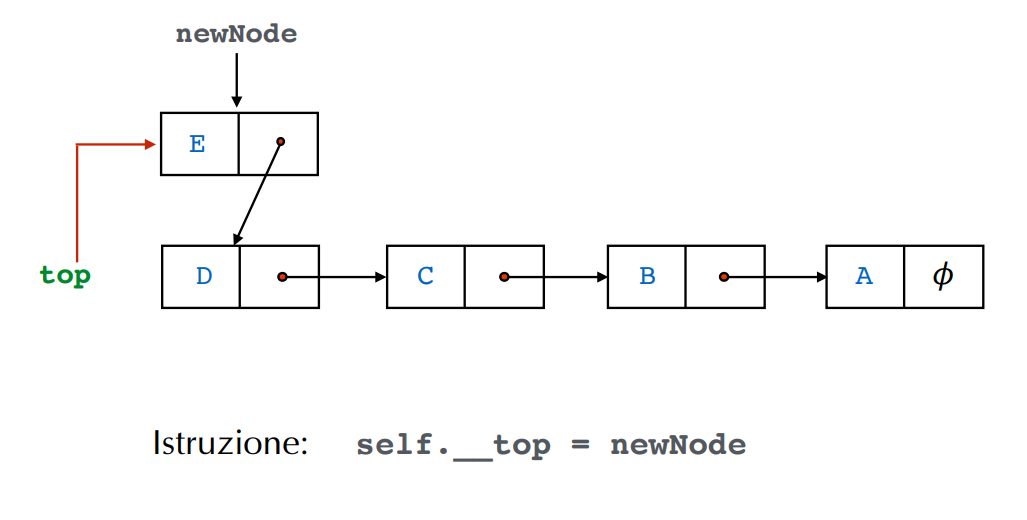
\includegraphics[width=8cm, height=5cm]{Screenshot 2024-11-11 175356.png} % Sostituisci con il nome del tuo file immagine
       % \caption{Graph Search}
    \end{minipage}
\end{figure}
\begin{figure}[H] % Usa 'H' per forzare la posizione qui
    \centering % Centra l'immagine
    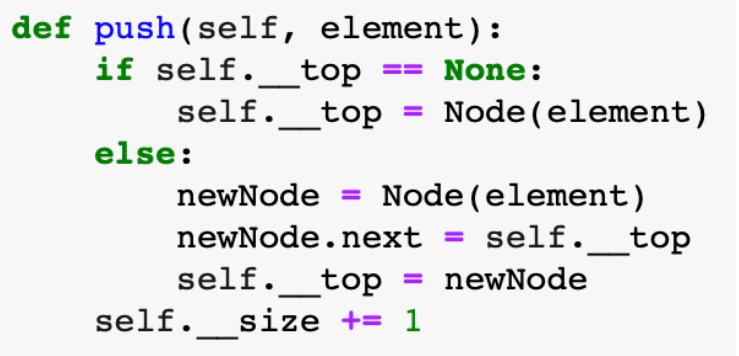
\includegraphics[width=8cm, height=4cm]{Screenshot 2024-11-11 175511.png} % Percorso dell'immagine
    \caption{Inserimento di un elemento (PUSH)} % Didascalia per l'immagine
    \label{fig:immagine} % Etichetta per riferimento
\end{figure}
\textbf{Estrazione di un elemento (POP)}
\begin{figure}[H]
    \begin{minipage}[b]{0.45\textwidth} % Prima figura a sinistra
        \centering
        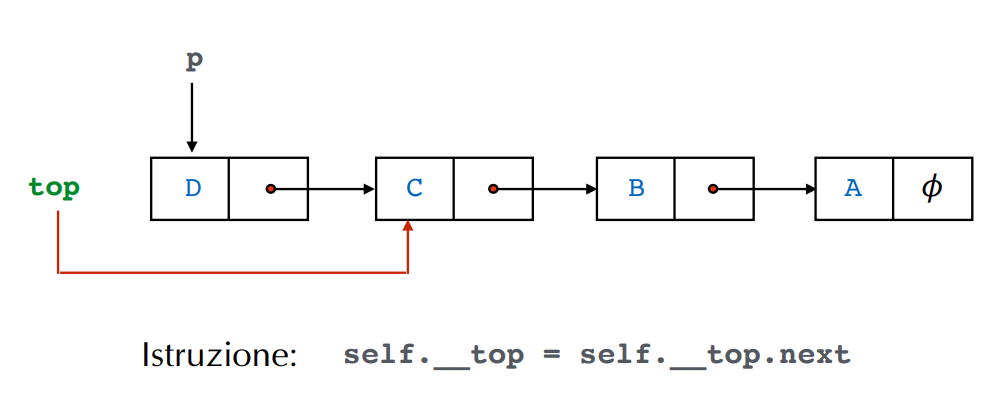
\includegraphics[width=8cm, height=5cm]{Screenshot 2024-11-11 175804.png} % Sostituisci con il nome del tuo file immagine
       % \caption{Tree Search}
    \end{minipage}
    \hfill
    \begin{minipage}[b]{0.45\textwidth} % Seconda figura a destra
        \centering
        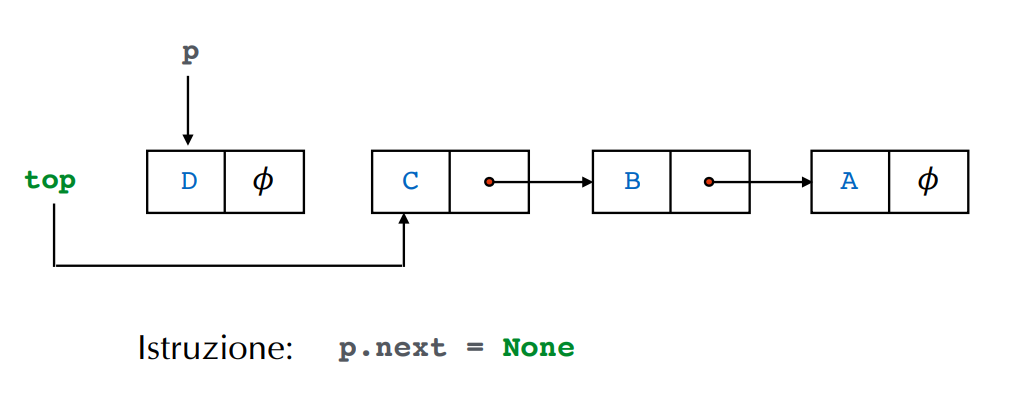
\includegraphics[width=8cm, height=5cm]{Screenshot 2024-11-11 175817.png} % Sostituisci con il nome del tuo file immagine
       % \caption{Graph Search}
    \end{minipage}
\end{figure}
\begin{figure}[H] % Usa 'H' per forzare la posizione qui
    \centering % Centra l'immagine
    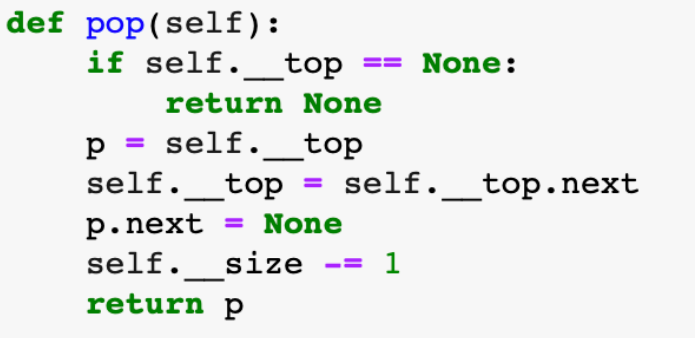
\includegraphics[width=8cm, height=4cm]{Screenshot 2024-11-11 175928.png} % Percorso dell'immagine
    \caption{Estrazione di un elemento (POP)} % Didascalia per l'immagine
    \label{fig:immagine} % Etichetta per riferimento
\end{figure}
\subsection{Le code}
Un altro importante tipo di dato astratto basato sul modello dei dati lista è la coda, una forma ristretta di lista in cui gli elementi vengono inseriti a un estremo, il retro (\textbf{tail}), ed estratti all'altro estremo, la fronte o testa (\textbf{head}). La politica di gestione è dunque la \textbf{First-In-First-Out (FIFO)}.\\
\textbf{Definizione della classe nodo}
\begin{figure}[H] % Usa 'H' per forzare la posizione qui
    \centering % Centra l'immagine
    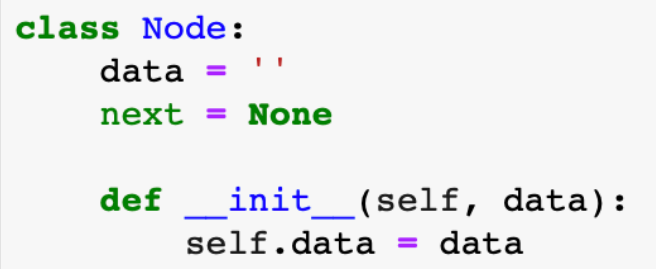
\includegraphics[width=8cm, height=3cm]{immagine_2024-11-11_180553488.png} % Percorso dell'immagine
    \caption{Definizione della classe nodo} % Didascalia per l'immagine
    \label{fig:immagine} % Etichetta per riferimento
\end{figure}
\textbf{Definizione della classe Queue}
\begin{figure}[H] % Usa 'H' per forzare la posizione qui
    \centering % Centra l'immagine
    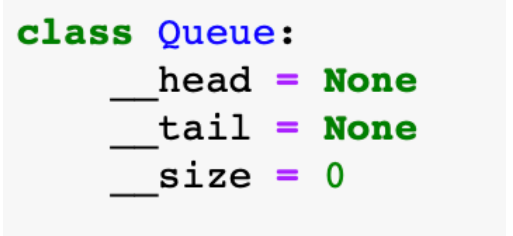
\includegraphics[width=8cm, height=3cm]{immagine_2024-11-11_180720906.png} % Percorso dell'immagine
    \caption{Definizione della classe Queue} % Didascalia per l'immagine
    \label{fig:immagine} % Etichetta per riferimento
\end{figure}
\noindent
\textbf{Inserimento di un elemento (Enqueue)}
\begin{figure}[H]
    \begin{minipage}[b]{0.45\textwidth} % Prima figura a sinistra
        \centering
        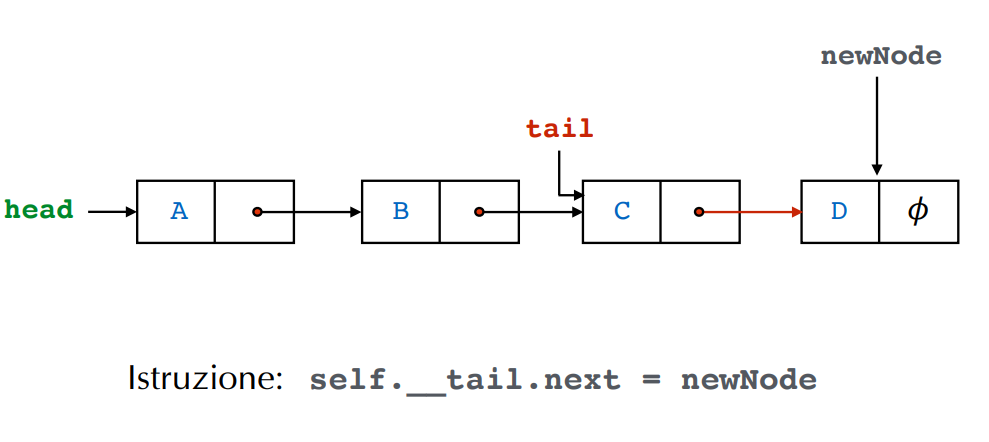
\includegraphics[width=8cm, height=4cm]{Screenshot 2024-11-11 180900.png} % Sostituisci con il nome del tuo file immagine
       % \caption{Tree Search}
    \end{minipage}
    \hfill
    \begin{minipage}[b]{0.45\textwidth} % Seconda figura a destra
        \centering
        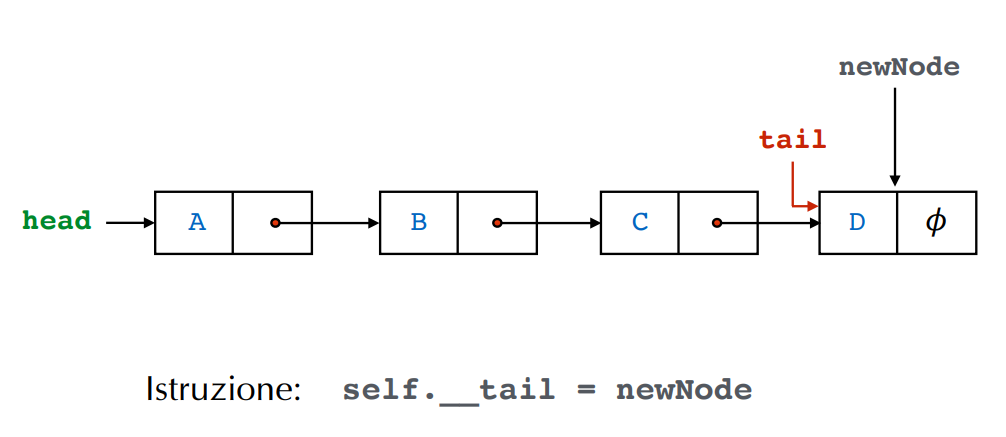
\includegraphics[width=8cm, height=4cm]{Screenshot 2024-11-11 180909.png} % Sostituisci con il nome del tuo file immagine
       % \caption{Graph Search}
    \end{minipage}
\end{figure}
\begin{figure}[H] % Usa 'H' per forzare la posizione qui
    \centering % Centra l'immagine
    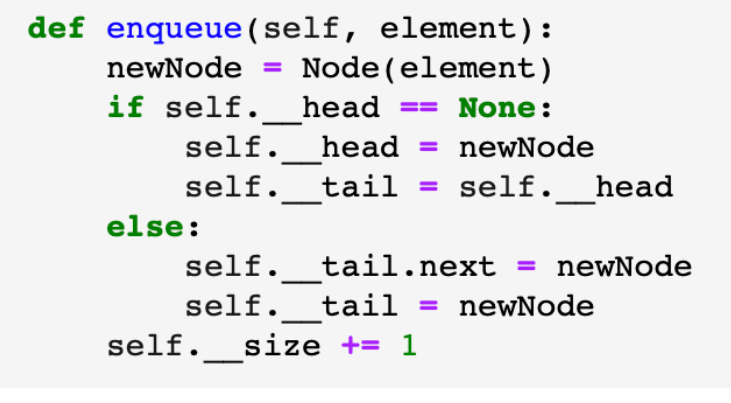
\includegraphics[width=10cm, height=4cm]{immagine_2024-11-11_181046674.png} % Percorso dell'immagine
    \caption{Inserimento di un elemento (Enqueue)} % Didascalia per l'immagine
    \label{fig:immagine} % Etichetta per riferimento
\end{figure}
\textbf{Estrazione di un elemento (Dequeue)}
\begin{figure}[H]
    \begin{minipage}[b]{0.45\textwidth} % Prima figura a sinistra
        \centering
        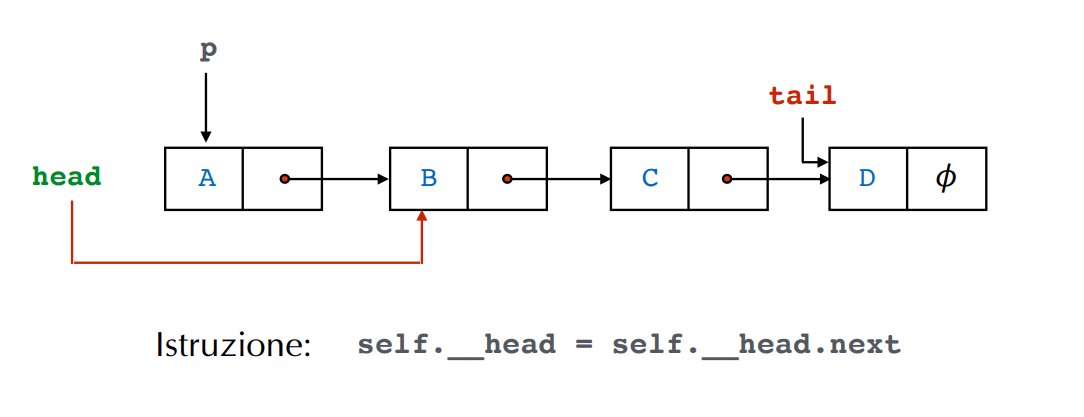
\includegraphics[width=8cm, height=4cm]{Screenshot 2024-11-11 181245.png} % Sostituisci con il nome del tuo file immagine
       % \caption{Tree Search}
    \end{minipage}
    \hfill
    \begin{minipage}[b]{0.45\textwidth} % Seconda figura a destra
        \centering
        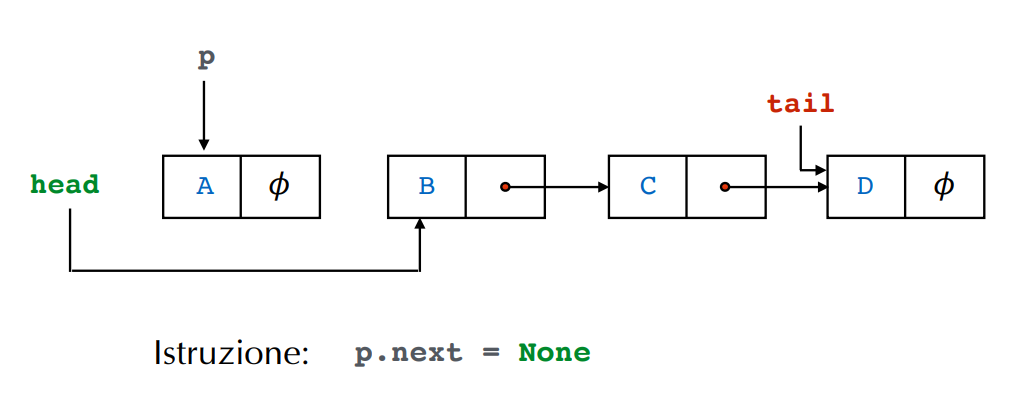
\includegraphics[width=8cm, height=4cm]{Screenshot 2024-11-11 181258.png} % Sostituisci con il nome del tuo file immagine
       % \caption{Graph Search}
    \end{minipage}
\end{figure}
\begin{figure}[H] % Usa 'H' per forzare la posizione qui
    \centering % Centra l'immagine
    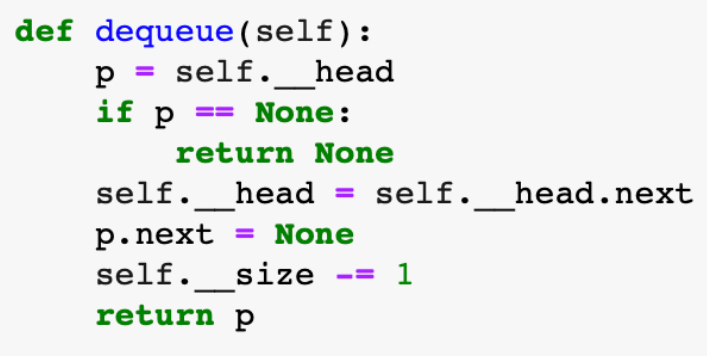
\includegraphics[width=10cm, height=4cm]{Screenshot 2024-11-11 181412.png} % Percorso dell'immagine
    \caption{Estrazione di un elemento (Dequeue)} % Didascalia per l'immagine
    \label{fig:immagine} % Etichetta per riferimento
\end{figure}
\vspace{200pt}
\subsection{Introduzioni agli algoritmi Python}
\subsubsection{Greedy Best-First Search}
L'algoritmo Greedy Best-First Search anche detto ricerca golosa, è un algoritmo che fa parte della ricerca euristica, brevemente la ricerca euristica utilizza una Queuing-FN (implementata nella frontiera) la quale ordina i nodi dal migliore al peggiore secondo la funzione di valutazione. Ovviamente il nodo scelto per l'espansione è quello la cui valutazione è "migliore". L'algoritmo Greedy ha \textbf{funzione di valutazione} $f=h$ (dove h è l'euristica, la quale ci aiuta a determinare la scelta sul nodo da espandere), infatti espande il nodo ritenuto più vicino a un obiettivo. Se h(n) = 0 vuol dire che lo stato n è un obiettivo. La ricerca golosa minimizza il costo stimato per raggiungere l'obiettivo. Nel problema della ricerca di un itinerario vogliamo raggiungere da una città di partenza, l'obiettivo a partire da Arad cercando di minimizzare il percorso. Questo algoritmo non è ne ottimale ne completo. \\
Nell'implementazione Python viene prima definito un dizionario che rappresenta il grafo degli stati, e un dizionario per la definizione dell'euristica.
\subsubsection{L'algoritmo A*}
L'algoritmo A*, è un algoritmo che fa parte della ricerca euristica, brevemente la ricerca euristica utilizza una Queuing-FN (implementata nella frontiera) la quale ordina i nodi dal migliore al peggiore secondo la funzione di valutazione. Ovviamente il nodo scelto per l'espansione è quello la cui valutazione è "migliore". Questo algoritmo ha come \textbf{funzione di valutazione} $f(n)=g(n)+h(n)$ ovvero la stima del costo del cammino a costo minimo dallo stato iniziale a un obiettivo, vincolato a passare per lo stato n. $g(n)$ rappresenta il "costo accumulato" dal nodo iniziale fino al nodo n, mentre $h(n)$ (l'euristica) in questo caso, è una stima del costo minimo per raggiungere l'obiettivo partendo da n.
Nel problema della ricerca di un itinerario vogliamo raggiungere da una città di partenza, l'obiettivo a partire da Arad cercando di minimizzare il percorso.
\subsubsection{Hill Climbing}
L'algoritmo Hill Climbing fa parte della categoria della ricerca locale. Ci sono problemi in cui lo stato obiettivo contiene tutte le informazioni rilevanti per la soluzione, infatti in questi casi il cammino verso l'obiettivo è irrilevante. Gli algoritmi di ricerca locale si muovono sulla superficie cercando i picchi più alti. Infatti il termine Hill Climbing deriva proprio da questo, infatti l'algoritmo segue sempre le salite più rapide. La versione che implementiamo in Python si chiama \textbf{First-Choice Hill Climbing}, esso dato lo stato corrente, sceglie casualmente un successore, e passa al nuovo stato se la valutazione di tale successore è migliore di quella dello stato corrente.
\subsubsection{Simulated Annealing}
L'algoritmo Hill Climbing fa parte della categoria della ricerca locale. Ci sono problemi in cui lo stato obiettivo contiene tutte le informazioni rilevanti per la soluzione, infatti in questi casi il cammino verso l'obiettivo è irrilevante. Gli algoritmi di ricerca locale si muovono sulla superficie cercando i picchi più alti.
L'algoritmo di Simulated Annealing prende il nome dall'analogia con il processo di ricottura in metallurgia che consiste nel ridurre gradualmente la temperatura di un materiale in modo da permettere alla sua struttura cristallina di raggiungere uno stato ad energia minima. Il Simulated Annealing comincia con valori alti di T comportandosi in modo simile ad una pura random search. Poi decrementa gradualmente il valore di T. Verso la fine dell'esecuzione i valori di T sono molto piccoli e perciò l'algoritmo si comporta in modo simile ad un normale hill-climber. Inoltre l'algoritmo accetta sempre nuovi punti se essi hanno una valutazione migliore del punto corrente. \textbf{La funzione tweak} viene utilizzata per scegliere random uno stato successore. \textbf{La funzione inizializza} serve per scegliere casualmente lo stato di partenza. \textbf{La funzione energia} è la funzione di valutazione.
\end{document}
